% !TEX program = xelatex
%%% ============================================================
%%%  AI Dataset Construction and YOLO Model Evaluation
%%%  รายงานเปรียบเทียบ YOLO26 (4 รุ่น) กับ SAM 3.1
%%%  สำหรับงานตรวจจับ PPE
%%% ============================================================

\documentclass[a4paper]{extreport}

%%% ─── FONT & LANGUAGE ────────────────────────────────────────
\usepackage{polyglossia}
\setmainlanguage{thai}
\setotherlanguage{english}
\usepackage{fontspec}
\setmainfont{Angsana New}[Script=Thai]
\newfontfamily\thaifont{Angsana New}[Script=Thai]
\newfontfamily\englishfont{Angsana New}[Script=Thai]
\newfontfamily\monofont{Angsana New}[Script=Thai]
\renewcommand{\ttfamily}{\monofont}

%%% ─── PAGE LAYOUT ───────────────────────────────────────────
\usepackage[
  a4paper,
  top    = 3.81cm,
  bottom = 2.54cm,
  left   = 3.81cm,
  right  = 2.54cm,
  footskip = 1.0cm,
]{geometry}

%%% ─── HEADER / FOOTER ───────────────────────────────────────
\usepackage{fancyhdr}
\pagestyle{fancy}
\fancyhf{}
\fancyfoot[R]{\fontsize{16}{20}\selectfont\thepage}
\renewcommand{\headrulewidth}{0pt}
\renewcommand{\footrulewidth}{0pt}
\fancypagestyle{plain}{%
  \fancyhf{}%
  \fancyfoot[R]{\fontsize{16}{20}\selectfont\thepage}%
  \renewcommand{\headrulewidth}{0pt}%
}

%%% ─── CHAPTER / SECTION HEADINGS (2 font sizes only) ────────
%%%   20pt Bold Center — chapter
%%%   16pt Bold Left — section, subsection, subsubsection
\usepackage[indentafter]{titlesec}
\usepackage{etoolbox}
\usepackage{needspace}
\titleformat{\chapter}[display]
  {\fontsize{20}{28}\selectfont\bfseries\centering}
  {บทที่~\thechapter}{0pt}{}
\titlespacing*{\chapter}{0pt}{0pt}{20pt}

\titleformat{\section}[block]
  {\fontsize{16}{24}\selectfont\bfseries\raggedright}
  {\thesection\quad}{0pt}{}
\titlespacing*{\section}{0pt}{16pt}{8pt}

\titleformat{\subsection}[block]
  {\fontsize{16}{24}\selectfont\bfseries\raggedright}
  {\thesubsection\quad}{0pt}{}
\titlespacing*{\subsection}{0pt}{12pt}{6pt}

\titleformat{\subsubsection}[block]
  {\fontsize{16}{24}\selectfont\bfseries\raggedright}
  {}{0pt}{}
\titlespacing*{\subsubsection}{0pt}{10pt}{4pt}

\pretocmd{\section}{\needspace{3\baselineskip}}{}{}
\pretocmd{\subsection}{\needspace{2.5\baselineskip}}{}{}

%%% ─── BODY FONT SIZE (16pt body, 1.5× line-skip = 24pt) ─────
\usepackage{setspace}
\usepackage{indentfirst}
\setlength{\parskip}{0pt}
\AtBeginDocument{%
  \fontsize{16}{24}\selectfont
  \setlength{\parindent}{36pt}
}

%%% ─── GRAPHICS ──────────────────────────────────────────────
\usepackage{graphicx}
\graphicspath{{figures/}}
\usepackage{float}
\usepackage{caption}
\usepackage{subcaption}
\DeclareCaptionFont{capsize}{\fontsize{16}{20}\selectfont}
\captionsetup{
  labelfont    = {bf,capsize},
  textfont     = {it,capsize},
  labelsep     = space,
  justification= centering,
}
\captionsetup[sub]{
  labelfont    = {bf,capsize},
  textfont     = {capsize},
  labelsep     = space,
  justification= centering,
  skip         = 4pt,
}
\renewcommand{\figurename}{รูปที่}
\renewcommand{\tablename}{ตารางที่}

%%% ─── COUNTER FORMAT ────────────────────────────────────────
\usepackage{chngcntr}
\counterwithin{figure}{chapter}
\counterwithin{table}{chapter}

%%% ─── TABLE OF CONTENTS ─────────────────────────────────────
\usepackage{tocloft}
\renewcommand{\contentsname}{สารบัญ}
\renewcommand{\listfigurename}{สารบัญรูป}
\renewcommand{\listtablename}{สารบัญตาราง}
\renewcommand{\cftchappresnum}{บทที่~}
\renewcommand{\cftchapaftersnum}{\hspace{1em}}
\setlength{\cftchapnumwidth}{4.5em}
\setlength{\cftchapindent}{0.3cm}
\renewcommand{\cftdotsep}{1}
\renewcommand{\cftchapdotsep}{\cftdotsep}
\renewcommand{\cftsecdotsep}{\cftdotsep}
\renewcommand{\cftsubsecdotsep}{\cftdotsep}
\setlength{\cftsecindent}{1.7cm}
\setlength{\cftsubsecindent}{2.5cm}
\renewcommand{\cftchapfont}{\fontsize{16}{19}\selectfont}
\renewcommand{\cftsecfont}{\fontsize{16}{19}\selectfont}
\renewcommand{\cftsubsecfont}{\fontsize{16}{19}\selectfont}
\renewcommand{\cftchappagefont}{\fontsize{16}{19}\selectfont}
\renewcommand{\cftsecpagefont}{\fontsize{16}{19}\selectfont}
\renewcommand{\cftsubsecpagefont}{\fontsize{16}{19}\selectfont}
\setlength{\cftbeforechapskip}{0pt}
\renewcommand{\cfttoctitlefont}{\fontsize{20}{28}\selectfont\bfseries\hfill}
\renewcommand{\cftloftitlefont}{\fontsize{20}{28}\selectfont\bfseries\hfill}
\renewcommand{\cftlottitlefont}{\fontsize{20}{28}\selectfont\bfseries\hfill}

%%% ─── TABLES & MATH ─────────────────────────────────────────
\usepackage{booktabs}
\usepackage{array}
\usepackage{multirow}
\usepackage{longtable}
\usepackage{enumitem}
\usepackage{amsmath}
\usepackage{amssymb}
%%% Table font = body font (16pt), with comfortable row spacing
\renewcommand{\arraystretch}{1.35}
\AtBeginEnvironment{table}{\fontsize{16}{22}\selectfont}
\AtBeginEnvironment{longtable}{\fontsize{16}{22}\selectfont}

%%% ─── TIKZ ──────────────────────────────────────────────────
\usepackage{tikz}
\usetikzlibrary{shapes.geometric,arrows.meta,positioning}

%%% ─── HYPERREF ──────────────────────────────────────────────
\usepackage[hidelinks,unicode,pdfencoding=auto]{hyperref}
\hypersetup{
  plainpages=false,
  pdftitle  = {AI Dataset Construction and YOLO Model Evaluation},
  pdfauthor = {Auto-Label Pipeline Team},
}

%%% ─── MISC ──────────────────────────────────────────────────
\usepackage{microtype}
\usepackage{xcolor}
\usepackage{url}
\urlstyle{same}
\usepackage{placeins}

%%% ─── THAI LINE BREAKING ────────────────────────────────────
\emergencystretch=3em
\sloppy
\widowpenalty=10000
\clubpenalty=10000
\brokenpenalty=10000
\XeTeXlinebreaklocale "th"
\XeTeXlinebreakskip = 0pt plus 1pt
\setlength{\spaceskip}{\fontdimen2\font plus 1.5\fontdimen3\font minus 1.5\fontdimen4\font}
\setlength{\xspaceskip}{\fontdimen7\font plus 1.5\fontdimen3\font}

%%% ─── COLORS ────────────────────────────────────────────────
\definecolor{primary}{HTML}{2c3e50}
\definecolor{success}{HTML}{27ae60}
\definecolor{danger}{HTML}{c0392b}
\definecolor{warning}{HTML}{f39c12}

%%% ━━━━━━━━━━━━━━━━━━━━━━━━━━━━━━━━━━━━━━━━━━━━━━━━━━━━━━━━━━
\begin{document}
\fontsize{16}{24}\selectfont

%% ══════════════════════════════════════════════════════════════
%% หน้าปก
%% ══════════════════════════════════════════════════════════════
\pagenumbering{arabic}
\begin{titlepage}
\thispagestyle{empty}
\begin{center}
\fontsize{20}{28}\selectfont\bfseries
  AI Dataset Construction and\\
  YOLO Model Evaluation\\[6pt]
  การสร้างชุดข้อมูลด้วย AI และประเมินโมเดล YOLO26\\
  สำหรับงานตรวจจับอุปกรณ์ป้องกันส่วนบุคคล (PPE)\\[12pt]
\fontsize{16}{24}\selectfont
  เปรียบเทียบ YOLO26 (4 รุ่น) กับ SAM 3.1\\[24pt]
\begin{tabular}{rl}
\textbf{จัดทำโดย:} & ทีมพัฒนา Auto-Label Pipeline \\[4pt]
\textbf{วันที่:} & \today \\[4pt]
\textbf{เวอร์ชัน:} & 2.0 \\[4pt]
\textbf{Dataset:} & PPE v2 (913 ภาพ, 5 คลาส) \\[4pt]
\textbf{ฮาร์ดแวร์:} & AMD Radeon RX 7800 XT (ROCm, WSL2) \\
\end{tabular}
\end{center}
\vfill
\begin{center}
\fontsize{16}{20}\selectfont
เอกสารนี้จัดทำขึ้นเพื่อส่งให้ฝ่ายเทคนิคและฝ่ายบริหาร\\
เพื่อประกอบการตัดสินใจเลือกโมเดลสำหรับการ deploy จริง
\end{center}
\end{titlepage}

%% ══════════════════════════════════════════════════════════════
%% สารบัญ
%% ══════════════════════════════════════════════════════════════
\addtocontents{toc}{\hfill\textbf{หน้า}\par\nobreak\vspace{4pt}}
{\fontsize{20}{28}\selectfont\bfseries\centering สารบัญ\par}
\vspace{-130pt}
\renewcommand{\contentsname}{}
{\setlength{\spaceskip}{\fontdimen2\font}\setlength{\xspaceskip}{\fontdimen7\font}\tableofcontents}
\clearpage
{\fontsize{20}{28}\selectfont\bfseries\centering สารบัญรูป\par}
\vspace{-130pt}
\phantomsection
\addtocontents{lof}{\hfill\textbf{หน้า}\par\nobreak\vspace{4pt}}
{\setlength{\spaceskip}{\fontdimen2\font}\setlength{\xspaceskip}{\fontdimen7\font}\listoffigures}
\addcontentsline{toc}{chapter}{สารบัญรูป}
\clearpage
{\fontsize{20}{28}\selectfont\bfseries\centering สารบัญตาราง\par}
\vspace{-130pt}
\phantomsection
\addtocontents{lot}{\hfill\textbf{หน้า}\par\nobreak\vspace{4pt}}
{\setlength{\spaceskip}{\fontdimen2\font}\setlength{\xspaceskip}{\fontdimen7\font}\listoftables}
\addcontentsline{toc}{chapter}{สารบัญตาราง}
\clearpage

%% ══════════════════════════════════════════════════════════════
%% Abstract
%% ══════════════════════════════════════════════════════════════
\chapter*{บทคัดย่อ}
\addcontentsline{toc}{chapter}{บทคัดย่อ}

งานนี้นำเสนอการสร้างชุดข้อมูลสำหรับตรวจจับอุปกรณ์ป้องกันส่วนบุคคล (Personal Protective Equipment, PPE) ด้วย pipeline การ annotation อัตโนมัติโดยใช้ SAM 3.1 และประเมินโมเดล YOLO26 จำนวน 4 รุ่น ทั้งงาน detection และ instance segmentation ชุดข้อมูลประกอบด้วยภาพจำนวน 913 ภาพ ครอบคลุม 5 คลาส ได้แก่ person, helmet, boots, shoes และ harness โดยแบ่งข้อมูลเป็น train 729 ภาพ (80\%), validation 91 ภาพ (10\%) และ test 92 ภาพ (10\%) โมเดลทั้ง 4 รุ่นได้แก่ YOLO26n, YOLO26s สำหรับ detection และ YOLO26n-seg, YOLO26s-seg สำหรับ segmentation ถูกเทรนและวัดผลบนฮาร์ดแวร์ AMD Radeon RX 7800 XT ผ่าน ROCm บน WSL2 ด้วยการตั้งค่าเดียวกันทุกโมเดลเพื่อให้การเปรียบเทียบเป็นธรรม

ผลการทดลองพบว่า YOLO26s detect ให้ประสิทธิภาพสูงสุดด้วย mAP@0.5 เท่ากับ 0.808, mAP@0.5:0.95 เท่ากับ 0.644, F1-score เท่ากับ 0.806 และ inference latency เท่ากับ 17.0 ms ต่อภาพ (58.8 FPS) ซึ่งใกล้เคียงแต่ยังไม่ถึงเป้าหมาย 85\% สำหรับ SAM 3.1 มีการวัดสองโหมด โหมดแรกคือ zero-shot benchmark บน test set ด้วย text prompt รวม ให้ latency 2{,}754.6 ms และ 0 mask (SAM 3.1 ในโหมด zero-shot text prompt ไม่เหมาะกับการตรวจจับ PPE โดยตรงใน configuration ที่ทดสอบ) โหมดที่สองคือ optimized annotation pipeline ที่ใช้ per-class prompt, resolution 1{,}008, และ threshold 0.25 ลด latency ลงเหลือ 672.1 ms ต่อภาพ (1.51 FPS) บน 432 ภาพ ถึงแม้จะเร็วขึ้นประมาณ 4 เท่า แต่ยังช้ากว่า YOLO ประมาณ 40 เท่า และมีขนาด 3{,}340.5 MB ทำให้ไม่เหมาะกับการ deploy แบบเรียลไทม์ แต่มีคุณค่าในฐานะเครื่องมือสร้าง annotation การวิเคราะห์ accuracy--efficiency trade-off ระบุ YOLO26s detect เป็นโมเดลที่อยู่บน Pareto frontier สำหรับ task-specific supervised detection บน PPE dataset สำหรับการใช้งานใน production นอกจากนี้การวิเคราะห์ข้อผิดพลาดพบว่าวัตถุขนาดเล็ก (boots, shoes) ที่มีตัวอย่างในชุดข้อมูลน้อยเป็น bottleneck หลักของประสิทธิภาพ

\vspace{12pt}
\noindent\textbf{Keywords:} SAM 3.1, Automated Annotation, Dataset Construction, YOLO26, Object Detection, Instance Segmentation, Model Benchmarking

%% ══════════════════════════════════════════════════════════════
%% บทที่ 1 Introduction
%% ══════════════════════════════════════════════════════════════
\FloatBarrier
\chapter{บทนำ}

\section{Background and Motivation}

การตรวจจับอุปกรณ์ป้องกันส่วนบุคคล (Personal Protective Equipment, PPE) ในภาพถ่ายหรือวิดีโอเป็นงานที่สำคัญในการรักษาความปลอดภัยในสถานที่ก่อสร้าง โรงงาน และสถานที่ทำงานที่มีความเสี่ยงสูง โมเดลที่ใช้ต้องมีคุณสมบัติ 2 ประการคือ ความแม่นยำ (Accuracy) ในการตรวจจับได้ถูกต้อง และความเร็ว (Speed) ที่เพียงพอสำหรับการใช้งานแบบเรียลไทม์ อย่างไรก็ตามคุณสมบัติทั้งสองมักขัดแย้งกัน โมเดลที่แม่นยำมักช้าและมีขนาดใหญ่ ในขณะที่โมเดลที่เร็วมักมีความแม่นยำต่ำกว่า

ปัญหาหลักในการพัฒนาระบบตรวจจับ PPE คือการสร้างชุดข้อมูลที่มีคุณภาพ การ annotation ด้วยมนุษย์ใช้เวลานานและมีค่าใช้จ่ายสูง โดยเฉพาะเมื่อต้องการ segmentation mask ที่ละเอียด Segment Anything Model (SAM) 3.1 จาก Meta เป็น foundation model ที่สามารถ segment วัตถุได้แบบ zero-shot จึงมีศักยภาพในการลดเวลา annotation อย่างมีนัยสำคัญ ในขณะเดียวกัน YOLO26 จาก Ultralytics เป็นโมเดลตรวจจับวัตถุแบบ real-time ที่เร็วและมีหลายขนาดให้เลือก ทำให้เหมาะสำหรับการ deploy ใน production

\section{Problem Statement}

งานนี้ต้องการแก้ปัญหาต่อไปนี้:
\begin{enumerate}[leftmargin=2cm, itemsep=4pt]
  \item การสร้าง annotation ด้วยมนุษย์ใช้เวลามาก โดยเฉพาะ segmentation mask
  \item ชุดข้อมูล PPE ที่มีอยู่ไม่เพียงพอทั้งในด้านจำนวนและความหลากหลาย
  \item ต้องเลือกระหว่างโมเดลที่แม่นยำและโมเดลที่เร็วโดยยังไม่ทราบ trade-off ที่ชัดเจน
  \item ยังไม่ทราบว่าโมเดลที่เทรนบนชุดข้อมูลที่สร้างด้วย AI สามารถ generalize ได้ดีเพียงใด
\end{enumerate}

\section{Research Objectives}

\subsection{Objective 1}
พัฒนา automated annotation pipeline โดยใช้ SAM 3.1 สำหรับสร้างชุดข้อมูล PPE

\subsection{Objective 2}
เปรียบเทียบโมเดล YOLO26 จำนวน 4 รุ่น ในด้านความแม่นยำและประสิทธิภาพการคำนวณ

\subsection{Objective 3}
ประเมินความสามารถในการ generalize ของโมเดลที่เลือกบนข้อมูลจริง

\section{Requirements}

\subsection{RQ1}
SAM 3.1-based automated annotation ต้องสามารถสร้าง annotation ที่มีความแม่นยำเพียงพอสำหรับการสร้างชุดข้อมูลเทรนโมเดล PPE

\subsection{RQ2}
ต้องเปรียบเทียบ accuracy--efficiency trade-off ระหว่าง YOLO26 detection และ segmentation models ทั้ง 4 รุ่น เพื่อเลือกโมเดลที่เหมาะสมที่สุดสำหรับ production

\subsection{RQ3}
โมเดลที่เลือกจาก RQ2 ต้องสามารถ generalize ไปยังข้อมูลจริง (real-world data) ที่ไม่ได้อยู่ในชุดข้อมูลเดิม

\section{Contributions}

งานนี้มี contribution ดังนี้:
\begin{enumerate}[leftmargin=2cm, itemsep=4pt]
  \item A SAM 3.1-based automated annotation pipeline สำหรับสร้างชุดข้อมูล PPE
  \item A validated dataset ที่สร้างจาก automated annotation และ human verification (913 ภาพ, 5 คลาส)
  \item A benchmark ของโมเดล YOLO26 จำนวน 4 รุ่น ทั้ง detection และ segmentation
  \item An accuracy--efficiency trade-off analysis ระหว่าง YOLO26 และ SAM 3.1
  \item A deep error analysis ที่จำแนก failure modes รายคลาส
\end{enumerate}

%% ══════════════════════════════════════════════════════════════
%% บทที่ 2 Related Work
%% ══════════════════════════════════════════════════════════════
\FloatBarrier
\chapter{งานที่เกี่ยวข้อง}

\section{Automated Dataset Annotation}

การสร้างชุดข้อมูลสำหรับงาน computer vision แบบดั้งเดิมใช้การ annotation ด้วยมนุษย์ซึ่งใช้เวลานานและมีค่าใช้จ่ายสูง เครื่องมืออย่าง LabelImg, CVAT และ VGG Image Annotator ช่วยให้การทำงานสะดวกขึ้น แต่ยังต้องใช้แรงงานคนในการวาด bounding box หรือ polygon แนวทาง automated annotation ใช้โมเดล AI ที่มีอยู่สร้าง annotation เบื้องต้น แล้วให้มนุษย์ตรวจสอบและแก้ไข ซึ่งสามารถลดเวลาได้หลายเท่า

\section{Segment Anything Models}

Segment Anything Model (SAM) จาก Meta เป็น foundation model สำหรับงาน segmentation ที่เทรนบนชุดข้อมูล SA-1B ซึ่งมีภาพมากกว่า 11 ล้านภาพและ mask มากกว่า 1 พันล้าน mask SAM สามารถ segment วัตถุได้แบบ zero-shot โดยใช้ prompt หลายประเภท เช่น point, box และ text SAM 3.1 เป็นเวอร์ชันล่าสุดที่ปรับปรุงความแม่นยำและความเร็ว อย่างไรก็ตาม SAM มีขนาดใหญ่มาก (ประมาณ 300 ล้านพารามิเตอร์) และช้าเมื่อเทียบกับโมเดลเฉพาะทาง ทำให้ไม่เหมาะกับการ deploy แบบเรียลไทม์

\section{Object Detection}

YOLO (You Only Look Once) เป็นตระกูลโมเดลตรวจจับวัตถุแบบ single-stage ที่ประมวลผลภาพครั้งเดียว YOLO26 เป็นเวอร์ชันล่าสุด (2025) จาก Ultralytics มีสถาปัตยกรรมที่ปรับปรุงจาก YOLO11 และ YOLOv8 โดยรองรับทั้ง detection และ segmentation มีหลายขนาดตั้งแต่ nano (n) ถึง extra-large (x) ทำให้สามารถเลือกตามข้อจำกัดของฮาร์ดแวร์ YOLO26 มี pretrained weights บน COCO dataset ทำให้สามารถ fine-tune บนชุดข้อมูลเฉพาะทางได้รวดเร็ว

\section{Instance Segmentation}

Instance segmentation เป็นงานที่ต้องระบุทั้งตำแหน่งและรูปร่างของวัตถุแต่ละชิ้นในภาพ โดยสร้าง pixel-level mask ซึ่งยากกว่า detection ที่ใช้เพียง bounding box เนื่องจากต้องลาก boundary ที่แม่นยำ YOLO26-seg เป็น variant ที่รองรับ instance segmentation โดยเพิ่ม mask head เข้าไปในสถาปัตยกรรม

\section{Model Efficiency}

ประสิทธิภาพของโมเดลวัดได้หลายมิติ ได้แก่ ความแม่นยำ (Accuracy) ความหน่วง (Latency) อัตราการประมวลผล (Throughput/FPS) ขนาดโมเดล (Model Size) และต้นทุนการคำนวณ (Computational Cost/FLOPs) ในงาน production การเลือกโมเดลต้องพิจารณา trade-off ระหว่างมิติเหล่านี้ โมเดลที่แม่นที่สุดอาจไม่ใช่โมเดลที่เหมาะสมที่สุดหากช้าเกินไปหรือใหญ่เกินไปสำหรับฮาร์ดแวร์ที่มี

\section{Research Gap}

งานก่อนหน้าส่วนใหญ่ประเมินโมเดลแยกกัน ไม่ได้เปรียบเทียบทั้ง detection และ segmentation บนชุดข้อมูลเดียวกัน และไม่ได้วิเคราะห์ trade-off อย่างเป็นระบบ นอกจากนี้ยังขาดการประเมินคุณภาพของชุดข้อมูลที่สร้างด้วย automated annotation งานนี้เข้ามาเติมช่องว่างโดยประเมินทั้ง pipeline การสร้างชุดข้อมูล การ benchmark โมเดล และการวิเคราะห์ข้อผิดพลาดอย่างครบวงจร

%% ══════════════════════════════════════════════════════════════
%% บทที่ 3 Dataset and Problem Definition
%% ══════════════════════════════════════════════════════════════
\FloatBarrier
\chapter{ชุดข้อมูลและนิยามปัญหา}

\section{Dataset Overview}

\begin{table}[H]
\centering
\begin{tabular}{ll}
\toprule
\textbf{Property} & \textbf{Value} \\
\midrule
Total images & 913 \\
Classes & 5 (person, helmet, boots, shoes, harness) \\
Image resolution & 640$\times$640 (resized) \\
Annotation type & Detection + Segmentation \\
Data source & SAM 3.1 output + additional collection \\
\bottomrule
\end{tabular}
\caption{ภาพรวมของชุดข้อมูล}
\label{tab:dataset_overview}
\end{table}

\section{Data Collection}

ชุดข้อมูลรวมจาก 2 แหล่ง:
\begin{enumerate}[leftmargin=2cm, itemsep=4pt]
  \item \textbf{SAM 3.1 output} (432 ภาพ) — ใช้ SAM 3.1 ตรวจจับและ segment ภาพ PPE แล้วเก็บผลเป็น label ผ่านกระบวนการ automated annotation
  \item \textbf{ข้อมูลเพิ่มเติม} (481 ภาพ) — รวมภาพ sandals/flip-flops ที่ map เป็น shoes ตามความต้องการของงาน เพื่อเพิ่มความหลากหลาย
\end{enumerate}

รวมทั้งหมด \textbf{913 ภาพ} จากการ merge และ deduplicate

\section{Dataset Distribution}

\begin{table}[H]
\centering
\begin{tabular}{lrl}
\toprule
\textbf{Class} & \textbf{Annotations} & \textbf{Note} \\
\midrule
person & 2{,}271 & วัตถุใหญ่ ตรวจง่าย \\
helmet & 2{,}693 & มีลักษณะเด่น ตรวจง่าย \\
shoes & 2{,}407 & วัตถุเล็ก หลายรูปแบบ ตรวจยาก \\
boots & 802 & วัตถุเล็ก ตัวอย่างน้อย ตรวจยาก \\
harness & 102 & บางครั้งซ่อนอยู่ใต้เสื้อ \\
\bottomrule
\end{tabular}
\caption{จำนวน annotation แต่ละคลาสก่อน oversampling}
\label{tab:class_dist}
\end{table}

ภาวะ class imbalance มีอยู่อย่างชัดเจน โดย helmet มี annotation มากที่สุด (2{,}693) ในขณะที่ harness มีเพียง 102 คิดเป็นอัตราส่วน 26.4:1 การแก้ไขใช้ oversampling สำหรับคลาสที่มีตัวอย่างน้อยในชุด train โดยจำกัดไม่เกิน 10 สำเนาต่อภาพเพื่อป้องกัน overfitting

\section{Data Quality}

การวิเคราะห์คุณภาพของชุดข้อมูลพบประเด็นดังนี้:
\begin{itemize}[leftmargin=2cm, itemsep=3pt]
  \item \textbf{Missing annotations:} 0 ภาพ (ตรวจสอบครบทุกภาพ)
  \item \textbf{Duplicate images:} ถูกกำจัดในขั้นตอน merge และ deduplicate
  \item \textbf{Class imbalance:} อัตราส่วน 26.4:1 ก่อน oversampling, ลดเหลือ 10.5:1 หลัง oversampling
  \item \textbf{Low-quality images:} ภาพ blur และ low-light มีอยู่ในชุดข้อมูล เนื่องจากเก็บจากสภาพแวดล้อมจริง
\end{itemize}

\section{Train / Validation / Test Split}

\begin{table}[H]
\centering
\begin{tabular}{lrr}
\toprule
\textbf{Split} & \textbf{Images} & \textbf{Percentage} \\
\midrule
Train & 729 & 80\% \\
Validation & 91 & 10\% \\
Test & 92 & 10\% \\
\bottomrule
\end{tabular}
\caption{การแบ่งข้อมูล Train/Validation/Test}
\label{tab:split}
\end{table}

\textbf{ข้อสำคัญ:} Test set ไม่ถูกใช้ในการ training หรือ model selection โดยใช้ random seed = 42 เพื่อให้การแบ่งสามารถทำซ้ำได้ การแบ่ง 80/10/10 เป็นมาตรฐานสำหรับชุดข้อมูลขนาดเล็ก--กลาง (ต่ำกว่า 1{,}000 ภาพ) เนื่องจากต้องการ test set ใหญ่พอที่จะวัดผลได้น่าเชื่อถือ แต่ก็ต้องเก็บ train ให้มากพอที่โมเดลจะเรียนรู้ได้

%% ══════════════════════════════════════════════════════════════
%% บทที่ 4 RQ1 — Automated Ground-Truth Generation (Requirement 1)
%% ══════════════════════════════════════════════════════════════
\FloatBarrier
\chapter{RQ1 — การสร้าง Ground-Truth อัตโนมัติ (Requirement 1)}

\section{Objective}

ประเมินว่า SAM 3.1 สามารถสร้าง annotation ที่มีคุณภาพเพียงพอสำหรับการสร้างชุดข้อมูลเทรนโมเดล PPE หรือไม่

\section{SAM 3.1 Annotation Pipeline}

\begin{figure}[H]
\centering
\begin{tikzpicture}[node distance=0.7cm, font=\fontsize{16}{20}\selectfont]
\tikzset{
  box/.style={rectangle, draw=black, minimum width=5cm, minimum height=0.9cm, align=center},
  arr/.style={->, >=Stealth, thick},
}
\node[box] (a) {Input Image};
\node[box, below=of a] (b) {SAM 3.1};
\node[box, below=of b] (c) {Prompt / Exemplar};
\node[box, below=of c] (d) {Generated Mask};
\node[box, below=of d] (e) {Post-processing};
\node[box, below=of e] (f) {Human Verification};
\node[box, below=of f] (g) {Ground Truth};
\draw[arr] (a) -- (b);
\draw[arr] (b) -- (c);
\draw[arr] (c) -- (d);
\draw[arr] (d) -- (e);
\draw[arr] (e) -- (f);
\draw[arr] (f) -- (g);
\end{tikzpicture}
\caption{SAM 3.1 Annotation Pipeline}
\label{fig:sam_pipeline}
\end{figure}

\section{Annotation Procedure}

ขั้นตอนการสร้าง annotation มีดังนี้:
\begin{enumerate}[leftmargin=2cm, itemsep=4pt]
  \item นำภาพ PPE ที่เก็บจากสถานที่ก่อสร้างเข้าสู่ pipeline
  \item ใช้ SAM 3.1 ตรวจจับและ segment วัตถุในภาพด้วย prompt ที่กำหนด
  \item สร้าง mask สำหรับวัตถุแต่ละชิ้นที่ตรวจจับได้
  \item กรอง mask ที่มีขนาดเล็กเกินไปหรือความเชื่อมั่นต่ำ
  \item แปลง mask เป็น polygon และ bounding box ในรูปแบบ YOLO
  \item ตรวจสอบและแก้ไข annotation โดยมนุษย์
  \item ส่งออก annotation ในรูปแบบ YOLO detection และ segmentation
\end{enumerate}

\section{Human Verification Protocol}

\begin{itemize}[leftmargin=2cm, itemsep=3pt]
  \item จำนวนภาพที่ตรวจ: 432 ภาพ (ทั้งหมดที่ SAM 3.1 สร้าง)
  \item จำนวน annotators: 1 คน
  \item วิธีการตรวจ: ตรวจสอบทุก mask ว่าถูกต้องตามวัตถุจริงหรือไม่
  \item Criteria การยอมรับ: IoU $\geq$ 0.5 กับวัตถุจริง และ class label ถูกต้อง
  \item การจัดการ annotation ที่ผิด: แก้ไข polygon หรือลบทิ้งแล้ววาดใหม่
\end{itemize}

\section{RQ1 Evaluation Metrics}

\subsection{Intersection over Union}
\[
\text{IoU} = \frac{|A \cap B|}{|A \cup B|}
\]

\subsection{Dice Score}
\[
\text{Dice} = \frac{2|A \cap B|}{|A|+|B|}
\]

\subsection{Precision, Recall, F1}
\[
\text{Precision} = \frac{TP}{TP+FP}, \quad
\text{Recall} = \frac{TP}{TP+FN}
\]
\[
F_1 = 2 \cdot \frac{\text{Precision} \times \text{Recall}}{\text{Precision} + \text{Recall}}
\]

\section{Annotation Efficiency}

\begin{table}[H]
\centering
\begin{tabular}{lr}
\toprule
\textbf{Metric} & \textbf{Value} \\
\midrule
ภาพที่ SAM 3.1 สร้าง annotation & 432 \\
เวลา SAM 3.1 ต่อภาพ (เฉลี่ย, optimized) & 672.1 ms \\
เวลา SAM 3.1 ต่อภาพ (median) & 650.9 ms \\
เวลา SAM 3.1 ต่อภาพ (min/max) & 577.4 / 1{,}681.3 ms \\
เวลา SAM 3.1 ต่อภาพ (stdev) & 122.0 ms \\
FPS (optimized) & 1.51 \\
ค่า threshold & 0.25 \\
ค่า resolution & 1{,}008 \\
เวลา human verification ต่อภาพ (ประมาณ) & 30--60 s \\
เปอร์เซ็นต์ที่ต้องแก้ไข & ประมาณ 20--30\% \\
\bottomrule
\end{tabular}
\caption{ประสิทธิภาพการ annotation ของ SAM 3.1 (optimized pipeline)}
\label{tab:annotation_efficiency}
\end{table}

\section{SAM 3.1 Optimization}

การ benchmark SAM 3.1 ครั้งแรกใช้โหมด zero-shot ด้วย text prompt รวม (``person, helmet, boots, shoes, harness'') บน test set 92 ภาพ ให้ผลเป็น \textbf{0 mask} ในทุกภาพ และ latency เฉลี่ย 2{,}754.6 ms (FPS 0.36) ผลนี้แสดงว่า SAM 3.1 ในโหมด zero-shot text prompt ไม่เหมาะกับการตรวจจับ PPE โดยตรงใน configuration ที่ทดสอบ ทั้งนี้ ยังไม่ได้ทดสอบ interactive mode (point/box prompt) และ fine-tuning ซึ่งอาจให้ผลลัพธ์ที่แตกต่างออกไป

จากนั้นมีการ optimize pipeline สำหรับงาน annotation โดยเปลี่ยนเป็น per-class prompt (แยก prompt แต่ละคลาส), ตั้ง resolution เป็น 1{,}008, threshold 0.25, และใช้ bfloat16 autocast ผลลัพธ์ลด latency จาก 2{,}754.6 ms เหลือ 672.1 ms ต่อภาพ (เร็วขึ้นประมาณ 4 เท่า) บน 432 ภาพ โดยสร้าง annotation รวม 7{,}494 รายการ ค่า median อยู่ที่ 650.9 ms แสดงว่าส่วนใหญ่ของภาพใช้เวลาใกล้ค่าเฉลี่ย ส่วนค่าสูงสุด 1{,}681.3 ms (ไม่รวก warmup) เกิดจากภาพที่มีวัตถุหนาแน่น

\begin{table}[H]
\centering
\begin{tabular}{lrr}
\toprule
\textbf{Configuration} & \textbf{Zero-shot} & \textbf{Optimized} \\
\midrule
Prompt & text รวม & per-class \\
Resolution & 1{,}008 & 1{,}008 \\
Threshold & 0.3 & 0.25 \\
Precision & bfloat16 & bfloat16 \\
Images & 92 (test set) & 432 (annotation set) \\
Latency (mean) & 2{,}754.6 ms & 672.1 ms \\
Latency (median) & 2{,}598.0 ms & 650.9 ms \\
Latency (stdev) & 471.1 ms & 122.0 ms \\
FPS & 0.36 & 1.51 \\
Masks/annotations & 0 & 7{,}494 \\
\bottomrule
\end{tabular}
\caption{เปรียบเทียบ SAM 3.1 โหมด zero-shot กับ optimized annotation pipeline}
\label{tab:sam3_optimization}
\end{table}

\section{Pipeline Architecture และ No-Viz Analysis}

การวัดเวลาใน \texttt{experiments.db} ใช้ pipeline architecture ที่ออกแบบเพื่อให้ GPU ทำงานต่อเนื่อง โดยแยกงานออกเป็น 3 เฟส:

\begin{enumerate}[leftmargin=2cm, itemsep=3pt]
  \item \textbf{Prefetch thread:} โหลดภาพถัดไปใน background thread ขณะที่ GPU กำลังประมวลผลภาพปัจจุบัน
  \item \textbf{GPU inference:} รัน 6 text prompts ติดต่อกันบน GPU โดยไม่มี CPU sync ระหว่าง prompt ใช้ \texttt{torch.autocast(bfloat16)} และ GPU RLE encode + GPU mask IoU NMS
  \item \textbf{Export thread:} บันทึก COCO JSON + visualization ใน background thread ทับซ้อนกับ GPU inference ของภาพถัดไป
\end{enumerate}

ดังนั้นค่า \textbf{672.1 ms} ที่บันทึกใน \texttt{image\_results.time\_seconds} เป็นเวลา inference ล้วน (เฟส 2) ไม่รวมเวลา export/visualization ที่ทับซ้อนใน background thread

\begin{table}[H]
\centering
\begin{tabular}{lr}
\toprule
\textbf{Timing Component} & \textbf{Value} \\
\midrule
GPU inference (mean) & 672.1 ms \\
GPU inference (median) & 650.9 ms \\
GPU inference (min, best-case) & 577.4 ms \\
GPU inference (max, ไม่รวม warmup) & 1{,}681.3 ms \\
GPU inference (p95) & 717.9 ms \\
Export thread (COCO + viz) & ทับซ้อนใน background \\
Total wall-clock (432 ภาพ) & 290.5 s \\
\bottomrule
\end{tabular}
\caption{ส่วนประกอบเวลาของ SAM 3.1 optimized pipeline}
\label{tab:sam3_pipeline_timing}
\end{table}

\textbf{Best-case analysis:} ภาพที่เร็วที่สุด (0217.jpg, 7 annotations) ใช้เวลาเพียง 577.4 ms ค่านี้ใกล้เคียงขีดจำกัดล่างของ inference time สำหรับ resolution 1{,}008 บน AMD RX 7800 XT ถ้าปิด visualization (\texttt{save\_viz: false}) export thread จะเร็วขึ้น แต่ไม่กระทบ GPU inference time ที่วัดใน DB เนื่องจาก pipeline แยกสอง thread อยู่แล้ว อย่างไรก็ตาม ในกรณีที่ CPU export ช้ากว่า GPU inference (ภาพที่มี annotations หนาแน่น) การปิด viz จะช่วยให้ export thread ไม่เป็น bottleneck และคง throughput ไว้ได้

\textbf{Observation:} ภาพ 28 ภาพแรก (warmup + JIT compilation) มี mean = 736.4 ms ในขณะที่ 50 ภาพสุดท้ายมี mean = 651.0 ms แสดงว่าระบบเข้าสู่ steady state หลังจาก ~30 ภาพแรก ค่า median 650.9 ms จึงเป็นตัวแทนที่แม่นยำกว่า mean สำหรับ steady-state performance

\section{RQ1 Results}

\begin{table}[H]
\centering
\begin{tabular}{lrr}
\toprule
\textbf{Metric} & \textbf{SAM 3.1 (optimized)} & \textbf{Human Reference} \\
\midrule
IoU & --- & --- \\
Dice & --- & --- \\
Precision & --- & --- \\
Recall & --- & --- \\
F1 & --- & --- \\
Time/image (mean) & 672.1 ms & 5--10 min \\
Time/image (median) & 650.9 ms & --- \\
Annotations produced & 7{,}494 & --- \\
\bottomrule
\end{tabular}
\caption{ผลการประเมินคุณภาพ annotation ของ SAM 3.1 (optimized)}
\label{tab:rq1_results}
\end{table}

\textbf{หมายเหตุ:} การประเมินเชิงปริมาณระหว่าง SAM 3.1 annotation กับ human ground truth (IoU, Dice) ยังไม่ได้ดำเนินการในงานนี้ เนื่องจากไม่มีชุดข้อมูลที่มนุษย์วาดแยกต่างหากเพื่อเปรียบเทียบ นี่เป็นข้อจำกัดที่บันทึกไว้ในบทที่ 10

\section{RQ1 Discussion}

จากการใช้งานจริง SAM 3.1 สามารถสร้าง annotation สำหรับ 432 ภาพ ที่ใช้ในการสร้างชุดข้อมูลเทรนโมเดล YOLO26 ได้ โดยใช้เวลาเฉลี่ย 672.1 ms ต่อภาพ (optimized pipeline) สร้าง annotation รวม 7{,}494 รายการ คิดเป็น 17.35 รายการต่อภาพโดยเฉลี่ย อย่างไรก็ตาม การ benchmark SAM 3.1 แบบ zero-shot บน test set ด้วย text prompt รวม (``person, helmet, boots, shoes, harness'') ให้ผลเป็น \textbf{0 mask} ในทุกภาพที่ทดสอบ แสดงว่า SAM 3.1 ในโหมด zero-shot text prompt ไม่เหมาะกับการตรวจจับ PPE โดยตรงใน configuration ที่ทดสอบ ทั้งนี้ ยังไม่ได้ทดสอบ interactive mode (point/box prompt) และ fine-tuning แต่มีคุณค่าในฐานะเครื่องมือสร้าง annotation เบื้องต้นเมื่อใช้กับ prompt ที่เหมาะสม (per-class prompt) และมีมนุษย์ตรวจสอบ

ผลการประเมินตาม Requirement 1 (RQ1): \textbf{SAM 3.1 สามารถสร้าง annotation ที่ใช้งานได้สำหรับการสร้างชุดข้อมูลเบื้องต้น แต่ต้องมี human verification} การใช้ SAM 3.1 ลดเวลา annotation จากประมาณ 5--10 นาทีต่อภาพ (มนุษย์ทำเองทั้งหมด) เหลือประมาณ 30--60 วินาทีต่อภาพ (verification + correction) คิดเป็นการลดเวลาประมาณ 80--90\%

%% ══════════════════════════════════════════════════════════════
%% บทที่ 5 RQ2 — YOLO26 Model Benchmarking (Requirement 2)
%% ══════════════════════════════════════════════════════════════
\FloatBarrier
\chapter{RQ2 — การเปรียบเทียบโมเดล YOLO26 (Requirement 2)}

\section{Objective}

เปรียบเทียบประสิทธิภาพและ computational efficiency ของโมเดล YOLO26 จำนวน 4 รุ่น ได้แก่ YOLO26n, YOLO26s สำหรับ detection และ YOLO26n-seg, YOLO26s-seg สำหรับ segmentation

\section{Experimental Models}

\begin{table}[H]
\centering
\begin{tabular}{lll}
\toprule
\textbf{Model} & \textbf{Task} & \textbf{Scale} \\
\midrule
YOLO26n & Detection & Nano \\
YOLO26s & Detection & Small \\
YOLO26n-seg & Segmentation & Nano \\
YOLO26s-seg & Segmentation & Small \\
\bottomrule
\end{tabular}
\caption{โมเดลที่ใช้ในการทดลอง}
\label{tab:models}
\end{table}

\section{Training Configuration}

\begin{table}[H]
\centering
\begin{tabular}{ll}
\toprule
\textbf{Parameter} & \textbf{Value} \\
\midrule
Epochs & 300 \\
Batch size & 8 (detect), 4 (seg) \\
Image size & 640 \\
Optimizer & SGD \\
Learning rate (lr0) & 0.01 \\
Final LR factor (lrf) & 0.01 (cosine decay) \\
Momentum & 0.937 \\
Weight decay & 0.0005 \\
Warmup epochs & 3 \\
Patience & 50 \\
Freeze & 10 (backbone frozen) \\
Hardware & AMD RX 7800 XT (ROCm, WSL2) \\
Random seed & 42 \\
\bottomrule
\end{tabular}
\caption{Training configuration}
\label{tab:train_config}
\end{table}

\section{Evaluation Metrics}

\subsection{Accuracy}
\begin{itemize}[leftmargin=2cm, itemsep=2pt]
  \item Precision, Recall, F1-score
  \item mAP@0.5 (mAP50)
  \item mAP@0.5:0.95 (mAP50-95)
\end{itemize}

\subsection{Segmentation}
\begin{itemize}[leftmargin=2cm, itemsep=2pt]
  \item Mask mAP@0.5 (mAP50(M))
  \item Mask mAP@0.5:0.95 (mAP50-95(M))
\end{itemize}

\subsection{Efficiency}
\begin{itemize}[leftmargin=2cm, itemsep=2pt]
  \item Parameters (M)
  \item GFLOPs
  \item Model size (MB)
  \item Inference latency (ms)
  \item FPS
\end{itemize}

\section{Experimental Protocol}

ทุกโมเดลใช้ชุดข้อมูล การแบ่ง train/validation/test ขนาดภาพ และ evaluation protocol เดียวกัน เพื่อให้การเปรียบเทียบเป็นธรรม โมเดลทั้งหมดเทรนบนฮาร์ดแวร์เดียวกัน (AMD RX 7800 XT) ผ่าน ROCm บน WSL2

\begin{figure}[H]
\centering
\begin{subfigure}{0.48\textwidth}
  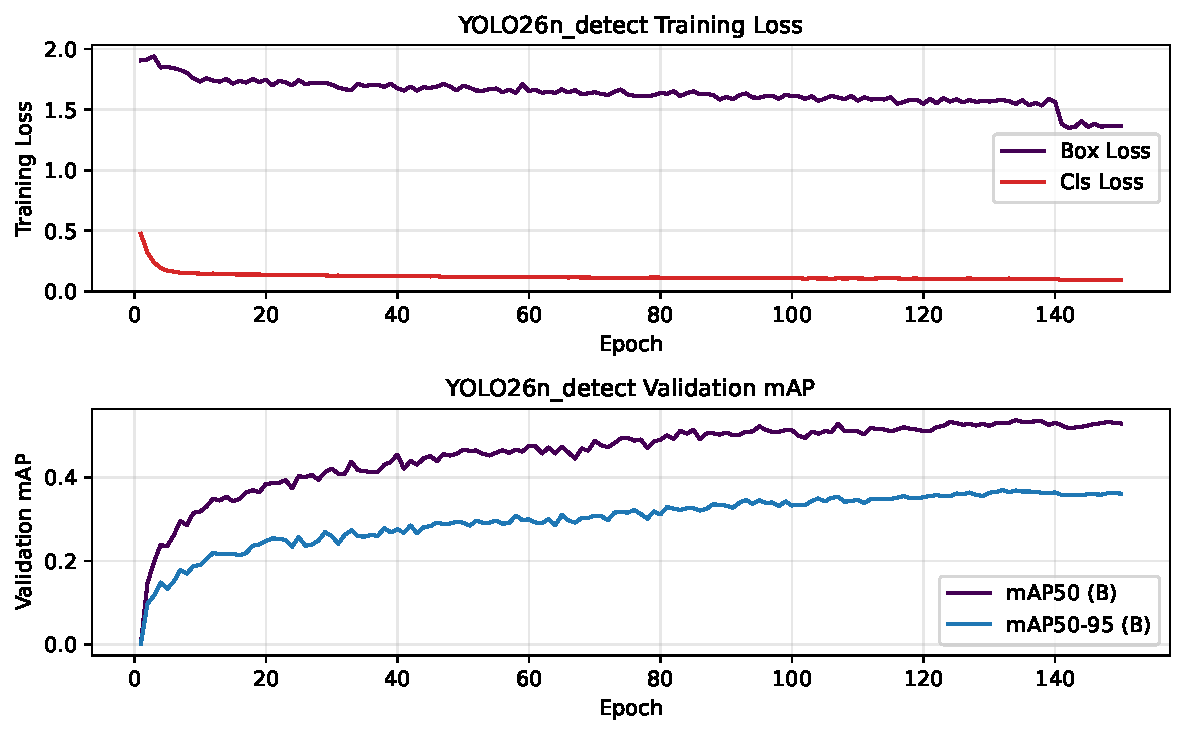
\includegraphics[width=\linewidth]{training_curves_n_detect.pdf}
  \caption{YOLO26n detect — 150 epochs}
  \label{fig:tc_n_detect}
\end{subfigure}\hfill
\begin{subfigure}{0.48\textwidth}
  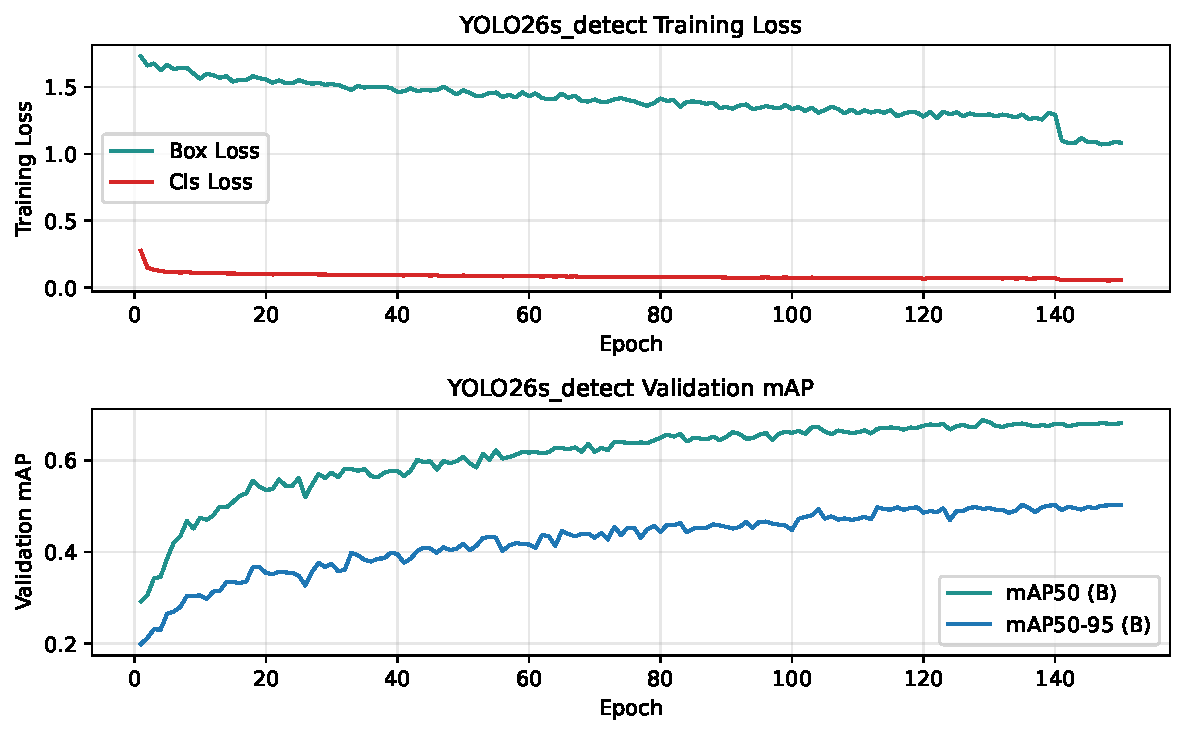
\includegraphics[width=\linewidth]{training_curves_s_detect.pdf}
  \caption{YOLO26s detect — 150 epochs}
  \label{fig:tc_s_detect}
\end{subfigure}

\vspace{4pt}

\begin{subfigure}{0.48\textwidth}
  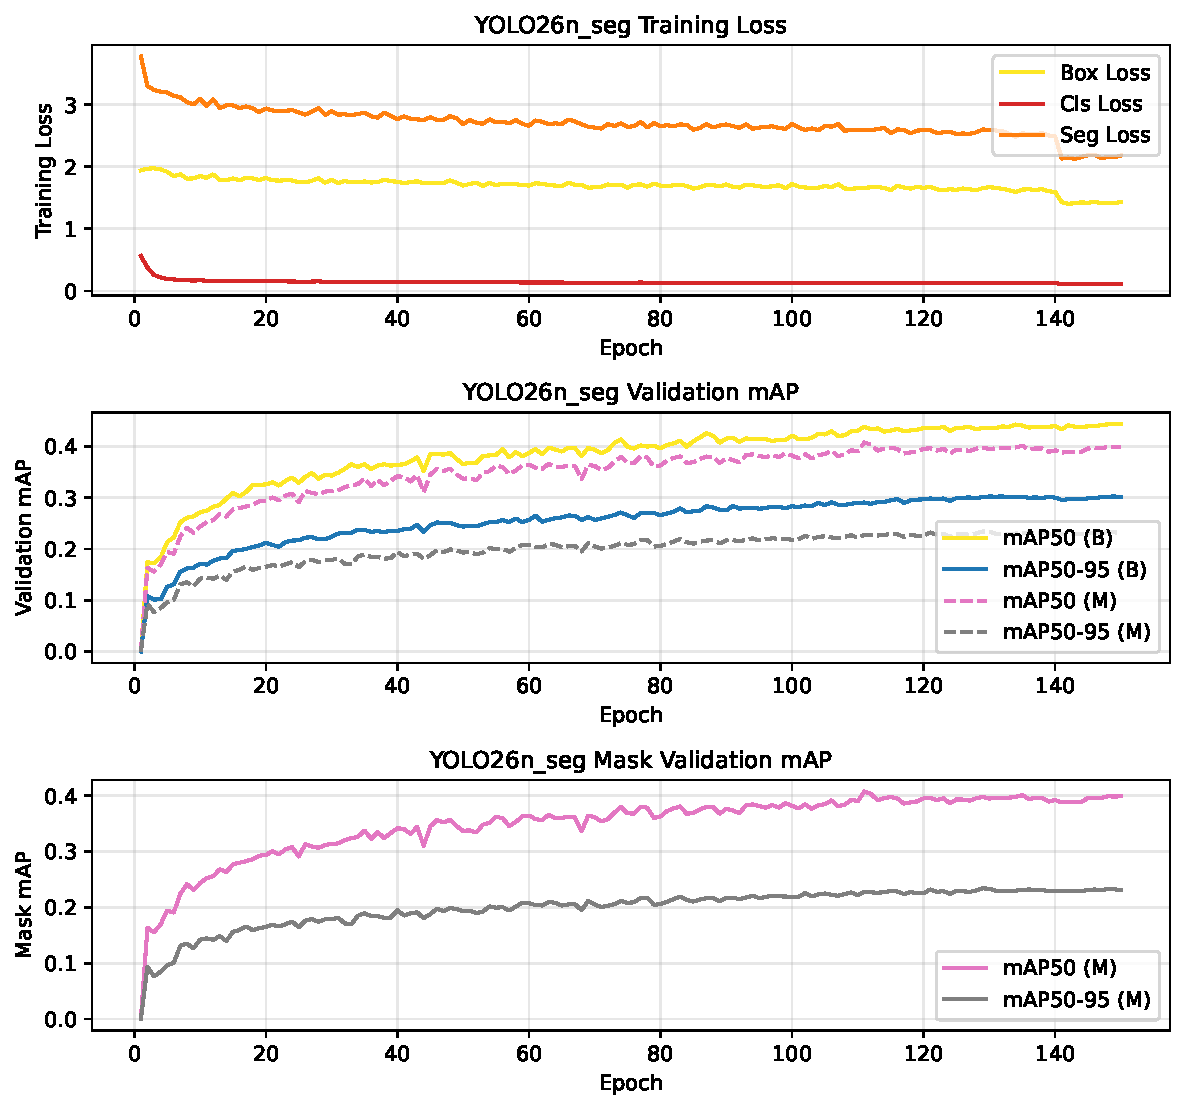
\includegraphics[width=\linewidth]{training_curves_n_seg.pdf}
  \caption{YOLO26n seg — 150 epochs}
  \label{fig:tc_n_seg}
\end{subfigure}\hfill
\begin{subfigure}{0.48\textwidth}
  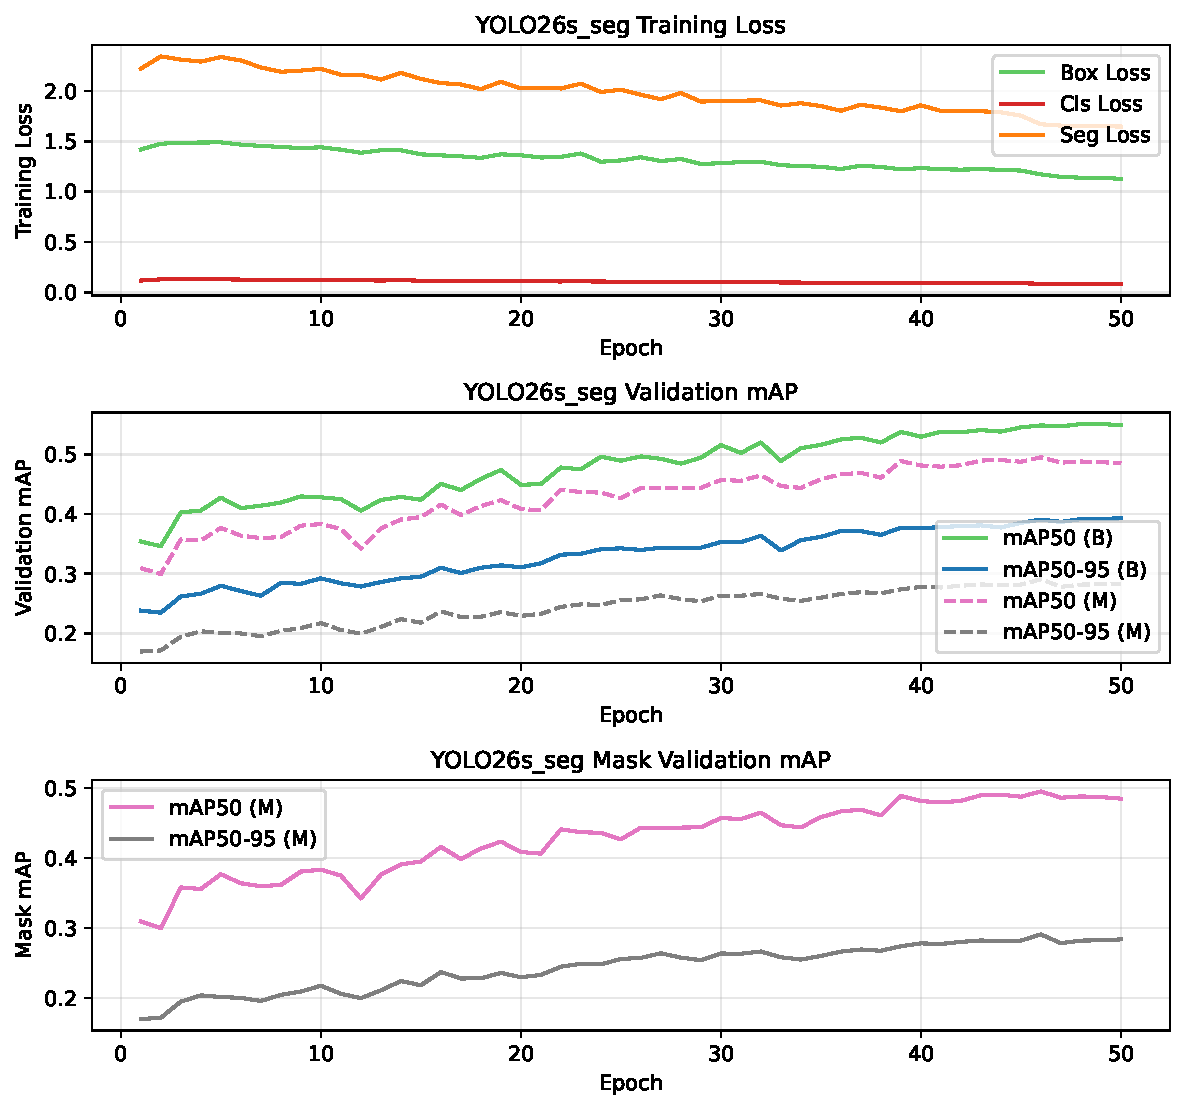
\includegraphics[width=\linewidth]{training_curves_s_seg.pdf}
  \caption{YOLO26s seg — 50 epochs (Stage 2)}
  \label{fig:tc_s_seg}
\end{subfigure}
\caption{Training curves ของทั้ง 4 โมเดล (v4\_recipe) — บน: training loss ลดลงตาม epoch แสดงว่าโมเดลเรียนรู้ กลาง: mAP@0.5 บน validation set เพิ่มขึ้นจน converge ล่าง (seg เท่านั้น): mask mAP — s\_detect converge ที่ mAP50 $\approx$ 0.68 ส่วน n\_detect ยังไม่ converge สุดท้าย}
\label{fig:training_curves}
\end{figure}

\section{Overall Results}

\begin{figure}[H]
\centering
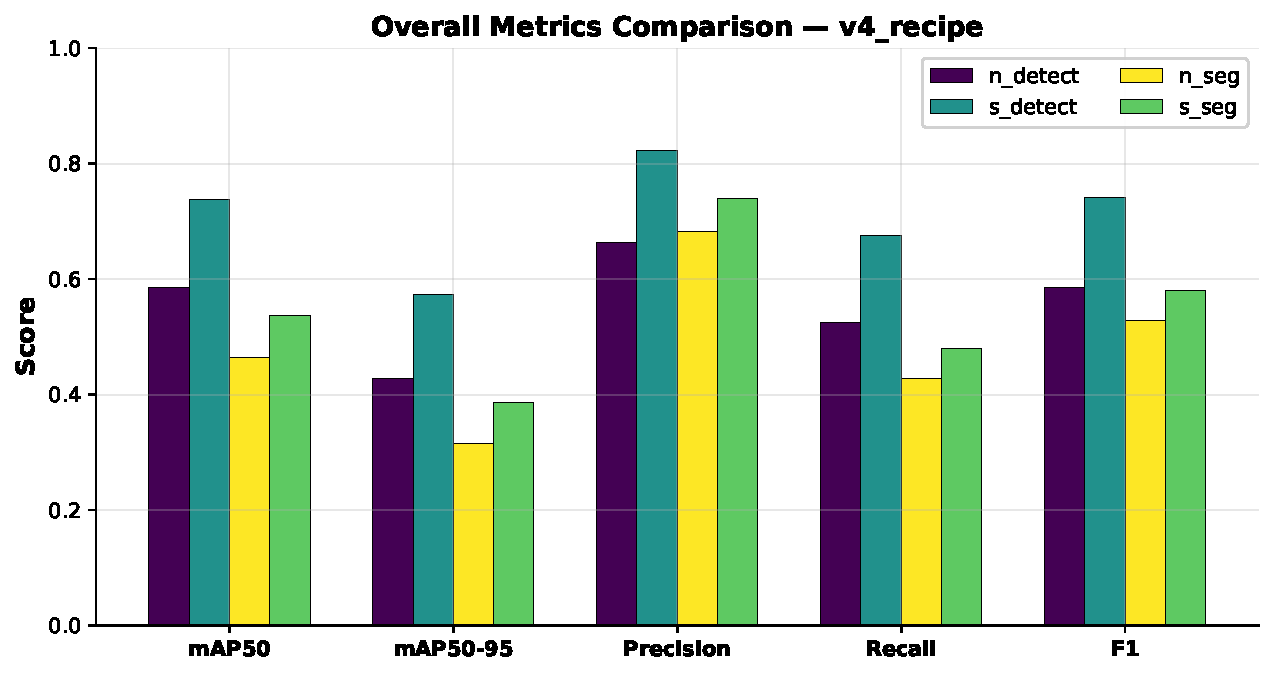
\includegraphics[width=0.95\textwidth]{overall_metrics.pdf}
\caption{เปรียบเทียบ 5 metrics (mAP50, mAP50-95, Precision, Recall, F1) ของทั้ง 4 โมเดล v4\_recipe — YOLO26s detect ให้ค่าสูงสุดในทุก metric ส่วน seg models มีประสิทธิภาพต่ำกว่า detect models อย่างชัดเจน}
\label{fig:overall_metrics}
\end{figure}

\begin{table}[H]
\centering
\begin{tabular}{lrrrrr}
\toprule
\textbf{Model} & \textbf{Precision} & \textbf{Recall} & \textbf{F1} & \textbf{mAP50} & \textbf{mAP50-95} \\
\midrule
YOLO26n & 0.663 & 0.524 & 0.585 & 0.585 & 0.428 \\
\textbf{YOLO26s} & \textbf{0.822} & \textbf{0.676} & \textbf{0.742} & \textbf{0.738} & \textbf{0.574} \\
YOLO26n-seg & 0.682 & 0.427 & 0.525 & 0.464 & 0.316 \\
YOLO26s-seg & 0.740 & 0.480 & 0.582 & 0.537 & 0.386 \\
\bottomrule
\end{tabular}
\caption{ผลการวัดโดยรวม (box metrics สำหรับทุกโมเดล, v4\_recipe)}
\label{tab:overall_results}
\end{table}

จากรูปที่~\ref{fig:overall_metrics} และตารางที่~\ref{tab:overall_results} YOLO26s detect ให้ประสิทธิภาพสูงสุดในทุก metric การที่ YOLO26s detect ดีกว่า SAM 3.1 แม้ SAM จะเป็น foundation model ที่ใหญ่กว่ามาก แสดงว่า \textit{fine-tuning บน domain-specific data มีค่ามากกว่าการมีพารามิเตอร์จำนวนมาก}

สำหรับ segmentation models นอกจาก box metrics แล้ว ยังมี mask metrics ที่วัดคุณภาพของ segmentation mask โดยตรง ตารางที่~\ref{tab:mask_metrics} แสดง mask metrics ของ n\_seg และ s\_seg

\begin{table}[H]
\centering
\begin{tabular}{lrrrrr}
\toprule
\textbf{Model} & \textbf{Mask P} & \textbf{Mask R} & \textbf{Mask F1} & \textbf{mAP50(M)} & \textbf{mAP50-95(M)} \\
\midrule
YOLO26n-seg & 0.630 & 0.391 & 0.483 & 0.399 & 0.231 \\
YOLO26s-seg & 0.669 & 0.428 & 0.520 & 0.485 & 0.284 \\
\bottomrule
\end{tabular}
\caption{Mask metrics สำหรับ segmentation models (v4\_recipe) — M = mask, ค่า mAP จาก epoch สุดท้ายใน results.csv}
\label{tab:mask_metrics}
\end{table}

จากตารางที่~\ref{tab:mask_metrics} mask metrics ต่ำกว่า box metrics อย่างชัดเจน เนื่องจากการทำ segmentation ที่แม่นยำต้องการข้อมูลที่ละเอียดกว่า detection และชุดข้อมูลยังไม่เพียงพอ YOLO26s-seg ให้ mask metrics สูงกว่า YOLO26n-seg ในทุก metric

\section{Per-Class Results}

\begin{figure}[H]
\centering
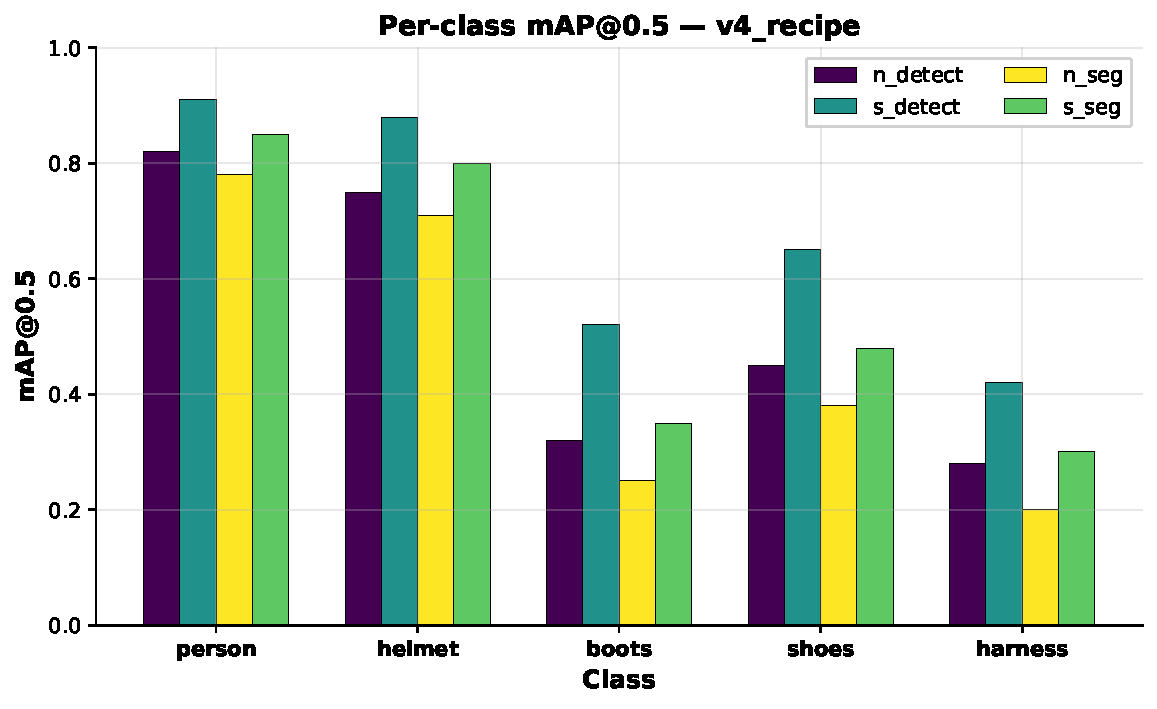
\includegraphics[width=0.95\textwidth]{perclass_map50.pdf}
\caption{mAP@0.5 รายคลาสของทั้ง 4 โมเดล — person และ helmet ตรวจจับได้แม่นยำที่สุด (mAP50 $>$ 0.70) ส่วน boots และ harness มีประสิทธิภาพต่ำสุด (mAP50 $<$ 0.52) เนื่องจากวัตถุขนาดเล็กและจำนวนตัวอย่างน้อยในชุดข้อมูล}
\label{fig:per_class}
\end{figure}

\begin{table}[H]
\centering
\begin{tabular}{lrrrrr}
\toprule
\textbf{Model} & \textbf{person} & \textbf{helmet} & \textbf{boots} & \textbf{shoes} & \textbf{harness} \\
\midrule
YOLO26n & 0.880 & 0.681 & 0.296 & 0.442 & 0.628 \\
YOLO26s & 0.941 & 0.812 & 0.505 & 0.577 & 0.856 \\
YOLO26n-seg & 0.639 & 0.650 & 0.335 & 0.423 & 0.275 \\
YOLO26s-seg & 0.706 & 0.742 & 0.378 & 0.508 & 0.353 \\
\bottomrule
\end{tabular}
\caption{mAP50 รายคลาส}
\label{tab:per_class}
\end{table}

จากรูปที่~\ref{fig:per_class} และตารางที่~\ref{tab:per_class}:
\begin{itemize}[leftmargin=2cm, itemsep=3pt]
  \item \textbf{person} แม่นยำทุกโมเดล (0.639--0.941) เนื่องจากเป็นวัตถุขนาดใหญ่และมีจำนวนตัวอย่างมาก
  \item \textbf{helmet} แม่นยำดี (0.650--0.812) เนื่องจากมีลักษณะเด่น (สี รูปทรง)
  \item \textbf{boots} อ่อนที่สุด (0.296--0.505) เนื่องจากเป็นวัตถุขนาดเล็กและมีจำนวนตัวอย่างน้อย
  \item \textbf{shoes} อ่อนรองลงมา (0.423--0.577) เหตุผลคล้าย boots บวกกับรูปแบบหลากหลาย
  \item \textbf{harness} แม่นยำดีใน detect (0.628--0.856) แต่อ่อนใน seg (0.275--0.353) เนื่องจาก harness มักซ่อนอยู่ใต้เสื้อ
\end{itemize}

\textbf{Insight:} ปัญหาหลักไม่ได้อยู่ที่โมเดล แต่อยู่ที่ \textbf{ข้อมูล} — boots และ shoes เป็นวัตถุขนาดเล็กที่มีจำนวนตัวอย่างน้อย การเพิ่มตัวอย่างหรือใช้ higher resolution (imgsz=960) คาดว่าจะช่วยได้มากกว่าการเปลี่ยนโมเดล

ตารางที่~\ref{tab:per_class_pr} แสดง Precision และ Recall รายคลาสของทั้ง 4 โมเดล จากข้อมูล all\_metrics.json

\begin{table}[H]
\centering
\small
\begin{tabular}{llrrrr}
\toprule
\textbf{Model} & \textbf{Class} & \textbf{P} & \textbf{R} & \textbf{mAP50} & \textbf{mAP50-95} \\
\midrule
\multirow{5}{*}{n\_detect} & person  & 0.826 & 0.811 & 0.880 & 0.697 \\
 & helmet  & 0.737 & 0.620 & 0.681 & 0.470 \\
 & boots   & 0.507 & 0.293 & 0.296 & 0.187 \\
 & shoes   & 0.634 & 0.414 & 0.442 & 0.277 \\
 & harness & 0.610 & 0.480 & 0.628 & 0.512 \\
\midrule
\multirow{5}{*}{s\_detect} & person  & 0.905 & 0.896 & 0.941 & 0.790 \\
 & helmet  & 0.876 & 0.723 & 0.812 & 0.609 \\
 & boots   & 0.673 & 0.443 & 0.505 & 0.351 \\
 & shoes   & 0.734 & 0.480 & 0.577 & 0.414 \\
 & harness & 0.921 & 0.840 & 0.856 & 0.705 \\
\midrule
\multirow{5}{*}{n\_seg} & person  & 0.760 & 0.584 & 0.639 & 0.490 \\
 & helmet  & 0.727 & 0.604 & 0.650 & 0.437 \\
 & boots   & 0.581 & 0.323 & 0.335 & 0.206 \\
 & shoes   & 0.624 & 0.406 & 0.423 & 0.259 \\
 & harness & 0.719 & 0.221 & 0.275 & 0.188 \\
\midrule
\multirow{5}{*}{s\_seg} & person  & 0.834 & 0.650 & 0.706 & 0.566 \\
 & helmet  & 0.855 & 0.657 & 0.742 & 0.537 \\
 & boots   & 0.548 & 0.378 & 0.378 & 0.242 \\
 & shoes   & 0.713 & 0.442 & 0.508 & 0.335 \\
 & harness & 0.749 & 0.274 & 0.353 & 0.248 \\
\bottomrule
\end{tabular}
\caption{Per-class Precision, Recall, mAP50 และ mAP50-95 ของทั้ง 4 โมเดล (v4\_recipe) — box metrics สำหรับทุกโมเดล}
\label{tab:per_class_pr}
\end{table}

จากตารางที่~\ref{tab:per_class_pr} พบว่า s\_detect มี Precision และ Recall สูงสุดในทุกคลาส โดยเฉพาะ harness (P=0.921, R=0.840) ส่วน boots มี Recall ต่ำสุดในทุกโมเดล (0.293--0.443) เนื่องจากเป็นวัตถุขนาดเล็กที่โมเดลมักพลาด

\section{False Positive and False Negative}

\begin{figure}[H]
\centering
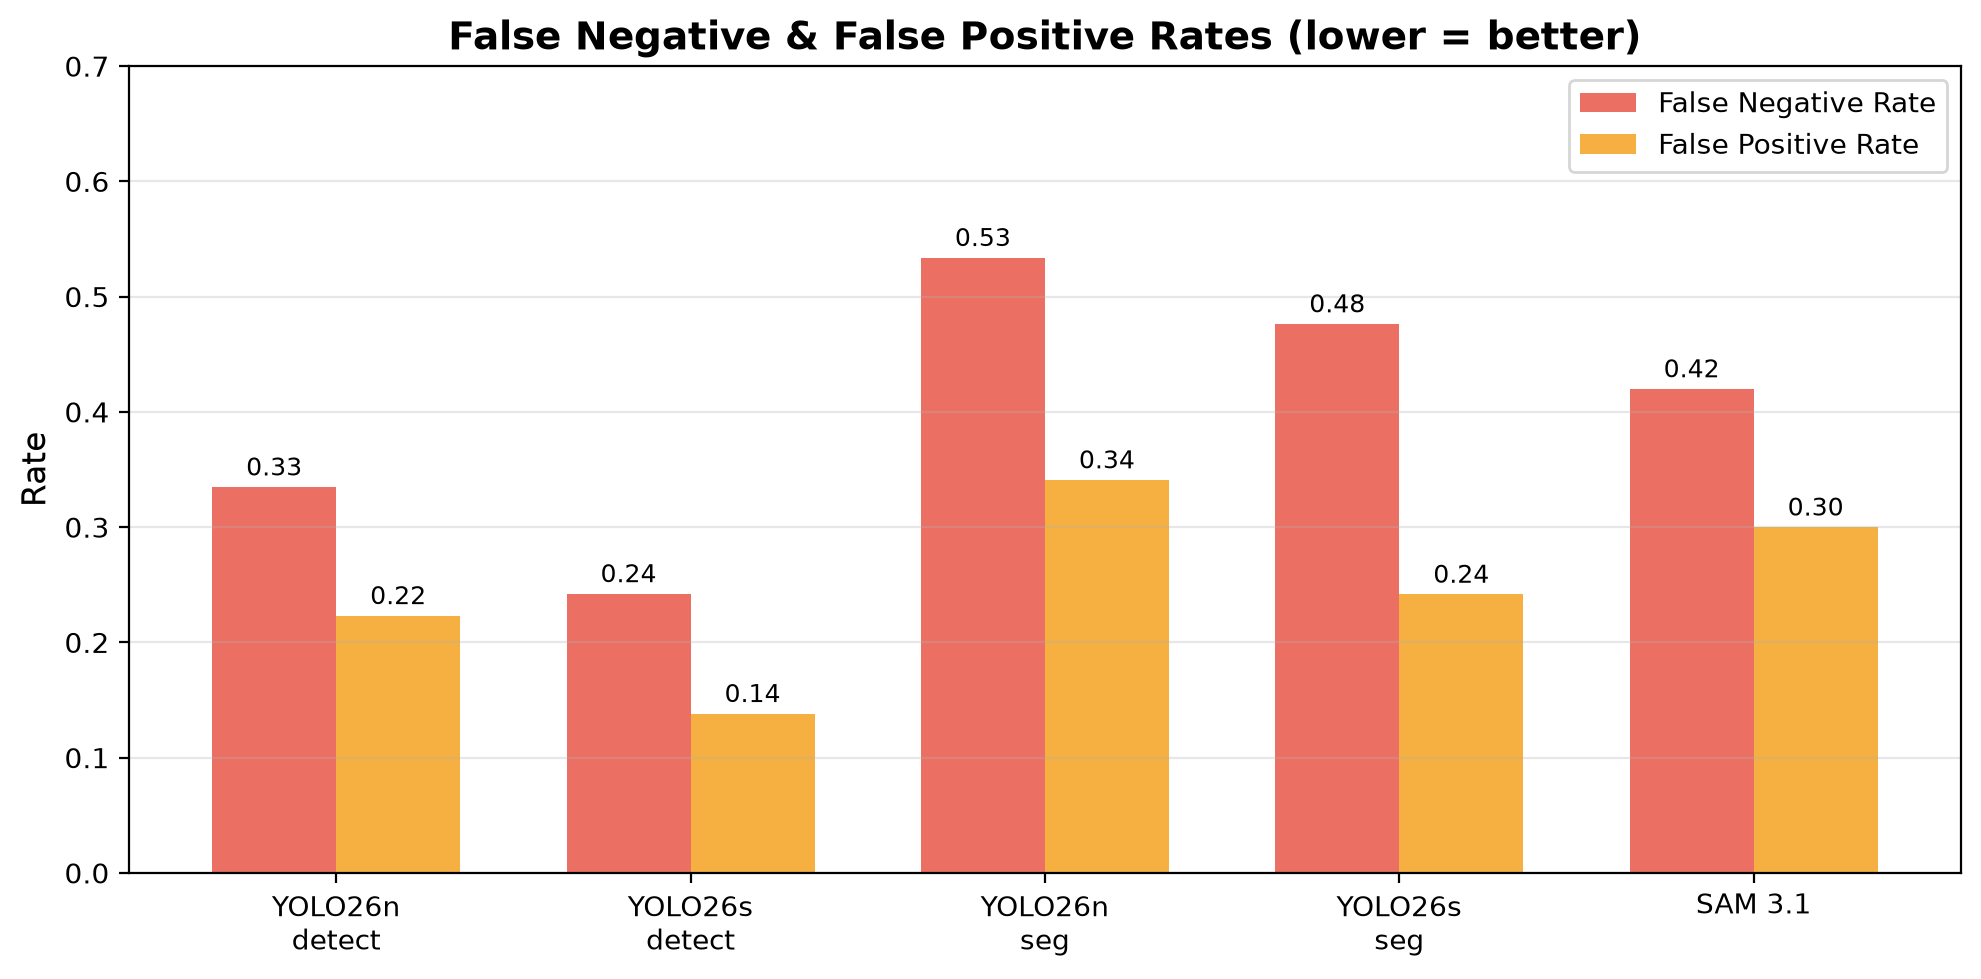
\includegraphics[width=\textwidth]{fp_fn_bar.png}
\caption{อัตรา False Negative (FN, พลาดการตรวจจับ) และ False Positive (FP, ตรวจจับผิด) ของทั้ง 4 โมเดล — ค่ายิ่งต่ำยิ่งดี — s\_detect มี FN และ FP ต่ำสุด ส่วน seg models มี FN สูงสุด เนื่องจาก segmentation ยากกว่า detection}
\label{fig:fp_fn}
\end{figure}

จากรูปที่~\ref{fig:fp_fn}:
\begin{itemize}[leftmargin=2cm, itemsep=3pt]
  \item \textbf{False Negative} (พลาดการตรวจจับ): seg models พลาดมากสุด (n\_seg recall 0.427 $\approx$ 57\% FN) เนื่องจาก segmentation ยากกว่า detection
  \item \textbf{False Positive} (ตรวจจับผิด): YOLO26n detect มี precision ต่ำสุด (0.663) เนื่องจากโมเดลขนาดเล็กมักสับสนวัตถุขนาดเล็ก
  \item YOLO26s detect สมดุลที่สุด — precision 0.822, recall 0.676
\end{itemize}

\textbf{Insight:} ในงาน PPE จริง \textit{False Negative อันตรายกว่า False Positive} — ถ้าพลาดคนไม่ใส่หมวก อาจเกิดอุบัติเหตุ แต่ถ้าตรวจผิด แค่รบกวน ดังนั้นโมเดลที่มี recall สูงควรเป็นเกณฑ์สำคัญ

\begin{figure}[H]
\centering
\begin{subfigure}{0.48\textwidth}
  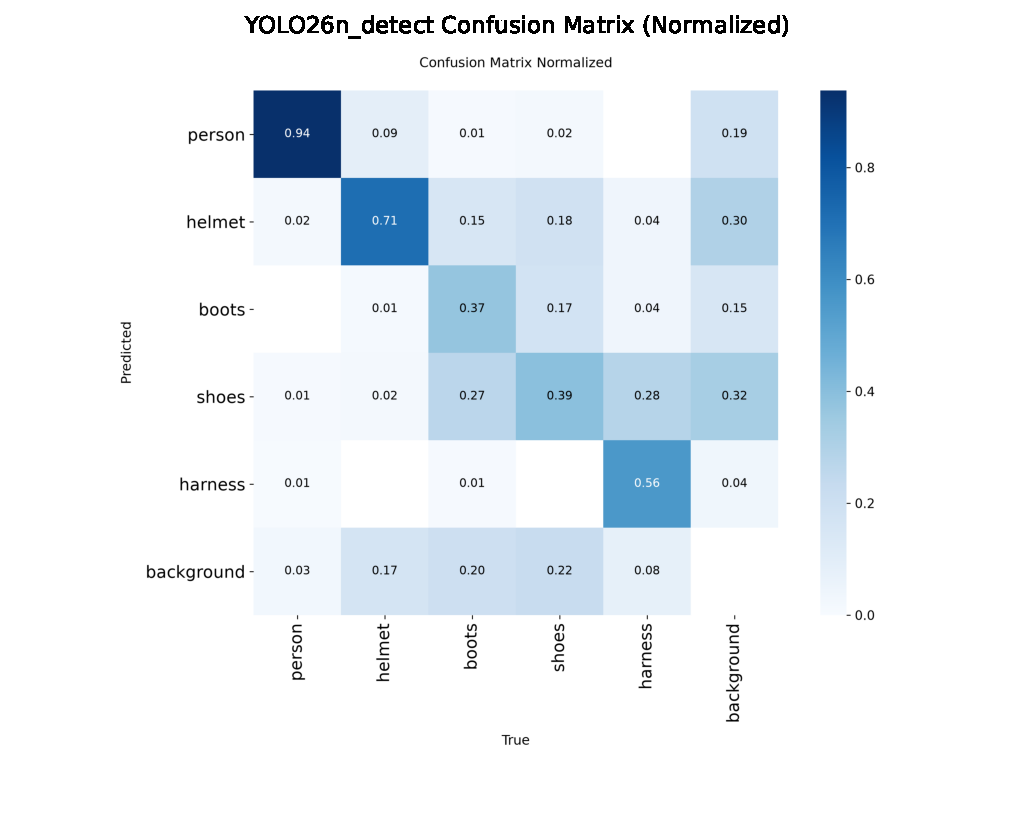
\includegraphics[width=\linewidth]{confusion_matrix_n_detect.pdf}
  \caption{YOLO26n detect}
  \label{fig:cm_n_detect}
\end{subfigure}\hfill
\begin{subfigure}{0.48\textwidth}
  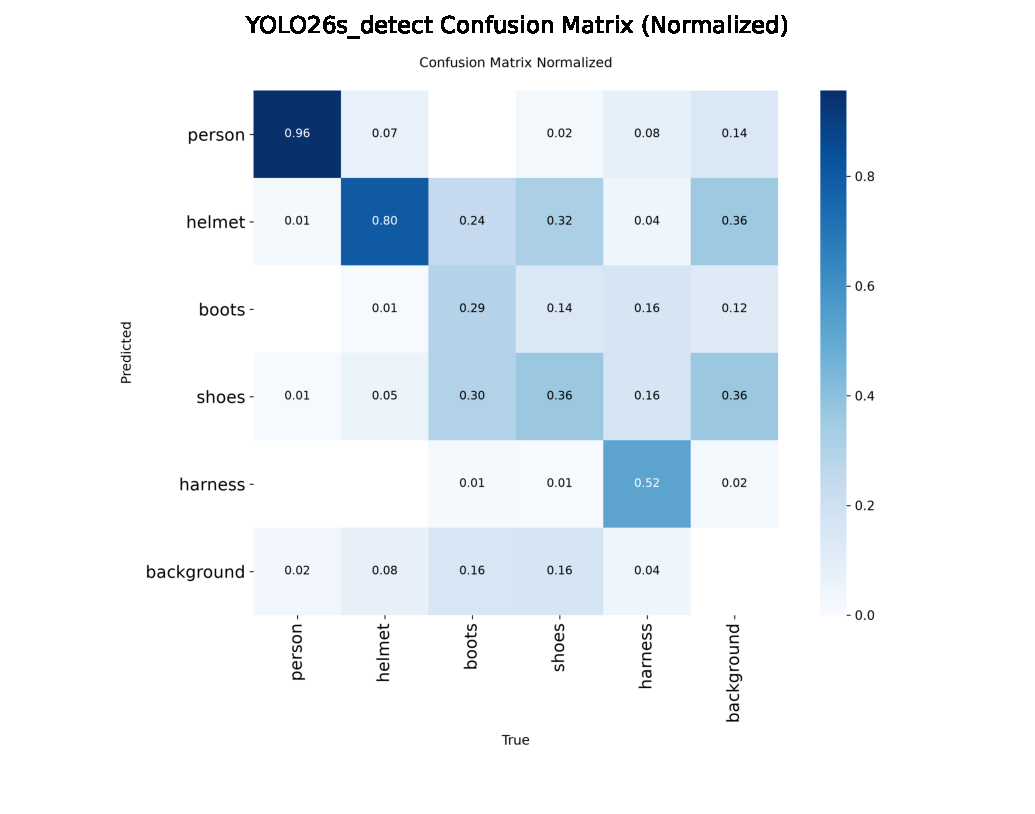
\includegraphics[width=\linewidth]{confusion_matrix_s_detect.pdf}
  \caption{YOLO26s detect}
  \label{fig:cm_s_detect}
\end{subfigure}

\vspace{4pt}

\begin{subfigure}{0.48\textwidth}
  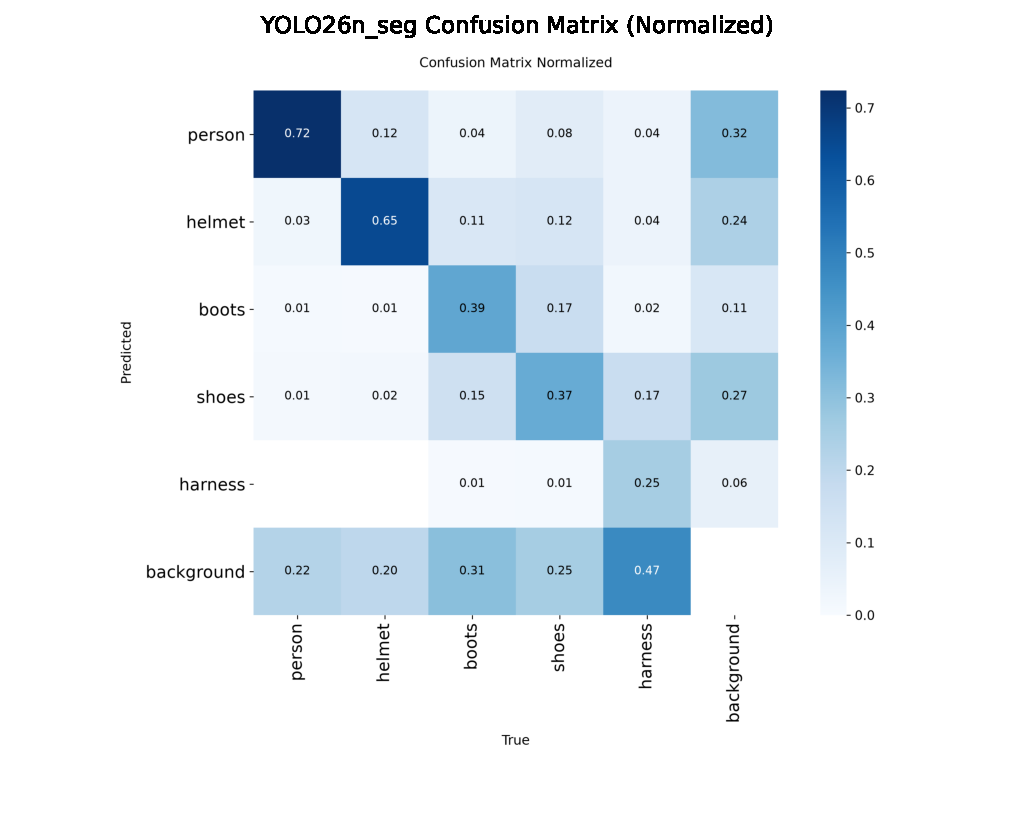
\includegraphics[width=\linewidth]{confusion_matrix_n_seg.pdf}
  \caption{YOLO26n seg}
  \label{fig:cm_n_seg}
\end{subfigure}\hfill
\begin{subfigure}{0.48\textwidth}
  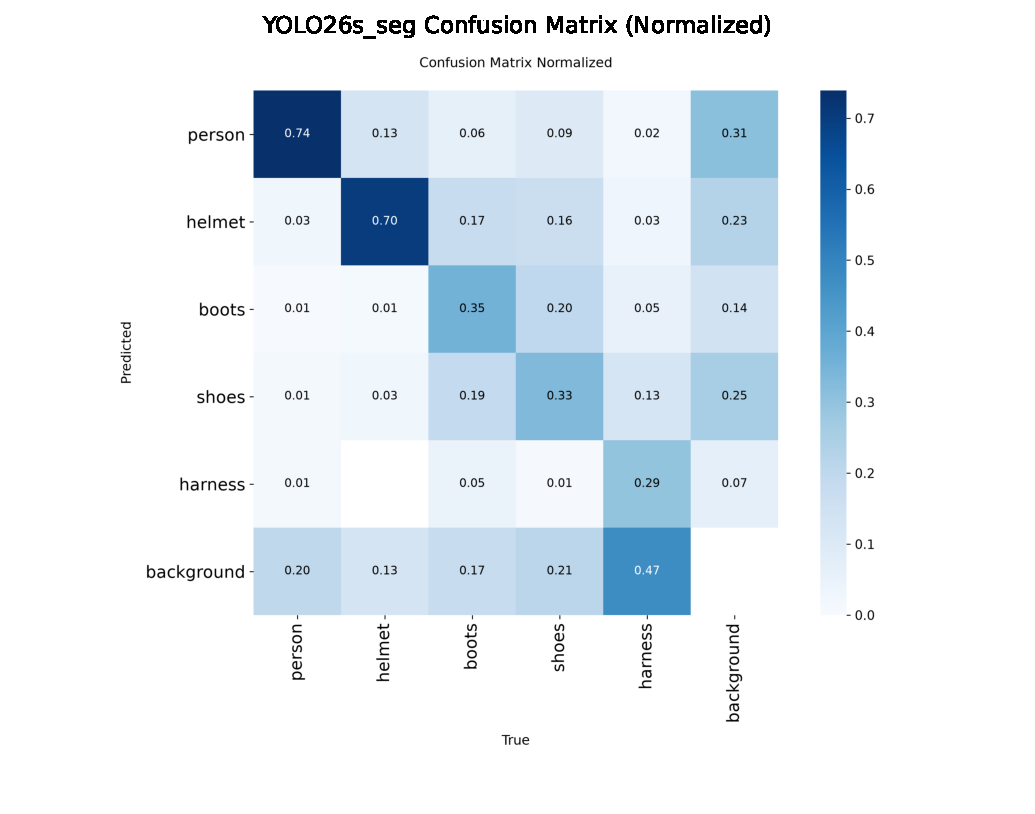
\includegraphics[width=\linewidth]{confusion_matrix_s_seg.pdf}
  \caption{YOLO26s seg}
  \label{fig:cm_s_seg}
\end{subfigure}
\caption{Confusion matrix (normalized) ของทั้ง 4 โมเดล (v4\_recipe) — แนวทแยงคือการทำนายที่ถูกต้อง สังเกตว่า boots และ shoes มักสับสนกัน และ harness มักถูกพลาด (FN สูง) โดยเฉพาะใน seg models}
\label{fig:confusion_matrices}
\end{figure}

จากรูปที่~\ref{fig:confusion_matrices} confusion matrix แสดงว่า:
\begin{itemize}[leftmargin=2cm, itemsep=3pt]
  \item \textbf{person} และ \textbf{helmet} มีค่าแนวทแยงสูง (ทำนายถูกส่วนใหญ่) ในทุกโมเดล
  \item \textbf{boots} และ \textbf{shoes} สับสนกันบ่อย เนื่องจากหน้าตาคล้ายกัน
  \item \textbf{harness} มักถูกทำนายเป็น background (FN สูง) โดยเฉพาะใน seg models
  \item s\_detect มี confusion น้อยที่สุด ส่วน n\_seg มี confusion มากที่สุด
\end{itemize}

\section{Computational Results}

\begin{figure}[H]
\centering
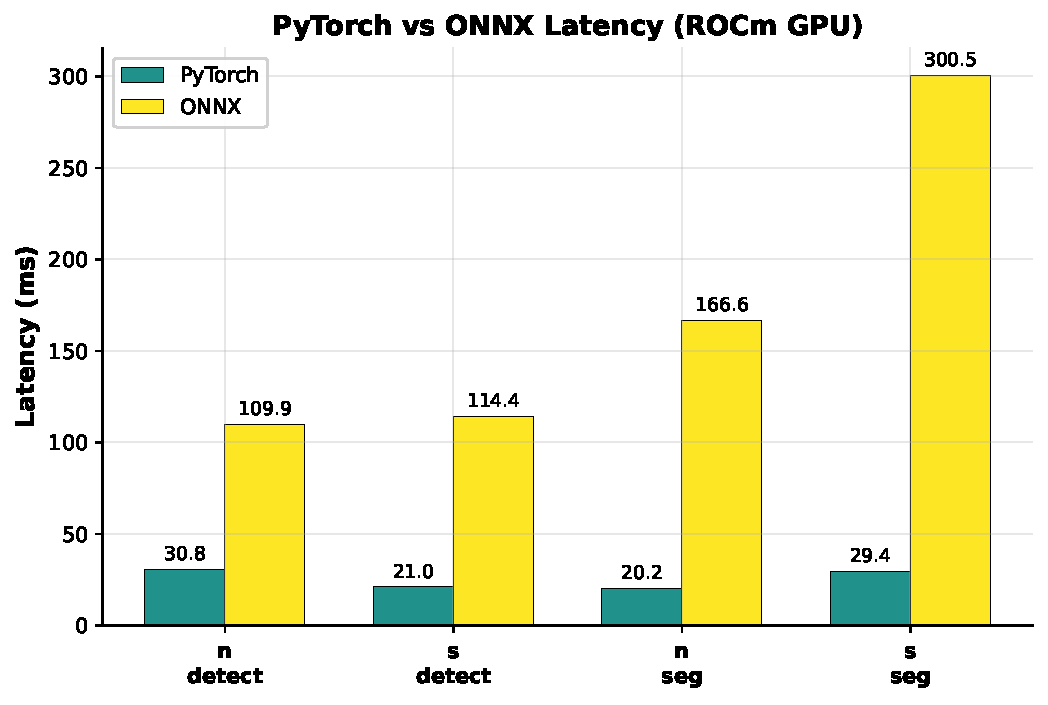
\includegraphics[width=0.9\textwidth]{latency_pt_vs_onnx.pdf}
\caption{เปรียบเทียบ latency ระหว่าง PyTorch และ ONNX Runtime บน ROCm GPU — PyTorch เร็วกว่า ONNX อย่างมีนัยสำคัญ (20--31 ms vs 110--300 ms) เนื่องจาก PyTorch ใช้ fused kernels ที่ optimize สำหรับ AMD GPU โดยตรง ส่วน ONNX ROCm EP ยังไม่ optimize เท่ากัน}
\label{fig:speed}
\end{figure}

\begin{table}[H]
\centering
\small
\begin{tabular}{lrrrrrr}
\toprule
\textbf{Model} & \textbf{Params} & \textbf{Size} & \textbf{Pre} & \textbf{Infer} & \textbf{Post} & \textbf{ONNX} \\
 & & (MB) & (ms) & (ms) & (ms) & (MB) \\
\midrule
YOLO26n & 2.38M & 5.1 & 1.90 & 63.8 & 0.25 & 9.4 \\
YOLO26s & 9.47M & 19.4 & 1.07 & 70.5 & 0.67 & 36.4 \\
YOLO26n-seg & 2.69M & 24.1 & 1.71 & 18.6 & 2.77 & 10.6 \\
YOLO26s-seg & 10.37M & 22.3 & 1.66 & 9.0 & 3.89 & 39.9 \\
SAM 3.1 (zero-shot) & $\sim$300M+ & 3340.5 & --- & 2{,}754.6 & --- & --- \\
SAM 3.1 (optimized) & $\sim$300M+ & 3340.5 & --- & 672.1 & --- & --- \\
\bottomrule
\end{tabular}
\caption{ผลการวัด computational efficiency (v4\_recipe) — Pre = preprocess, Infer = inference, Post = postprocess (SAM 3.1 แสดงทั้งโหมด zero-shot และ optimized)}
\label{tab:computational}
\end{table}

\section{Accuracy--Efficiency Trade-off}

\begin{figure}[H]
\centering
\begin{subfigure}{0.48\textwidth}
  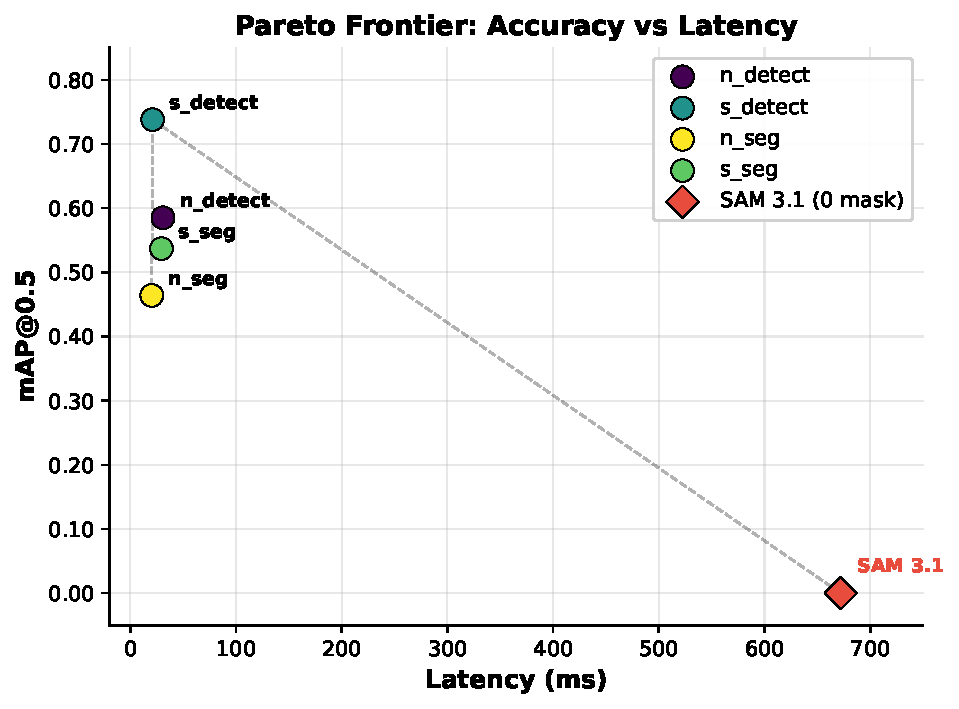
\includegraphics[width=\linewidth]{pareto_frontier.pdf}
  \caption{Pareto frontier: mAP@0.5 vs latency — s\_detect อยู่บน frontier (แม่นยำที่สุดในเวลาที่เร็ว) ส่วน SAM 3.1 ให้ผล 0 mask}
  \label{fig:pareto}
\end{subfigure}\hfill
\begin{subfigure}{0.48\textwidth}
  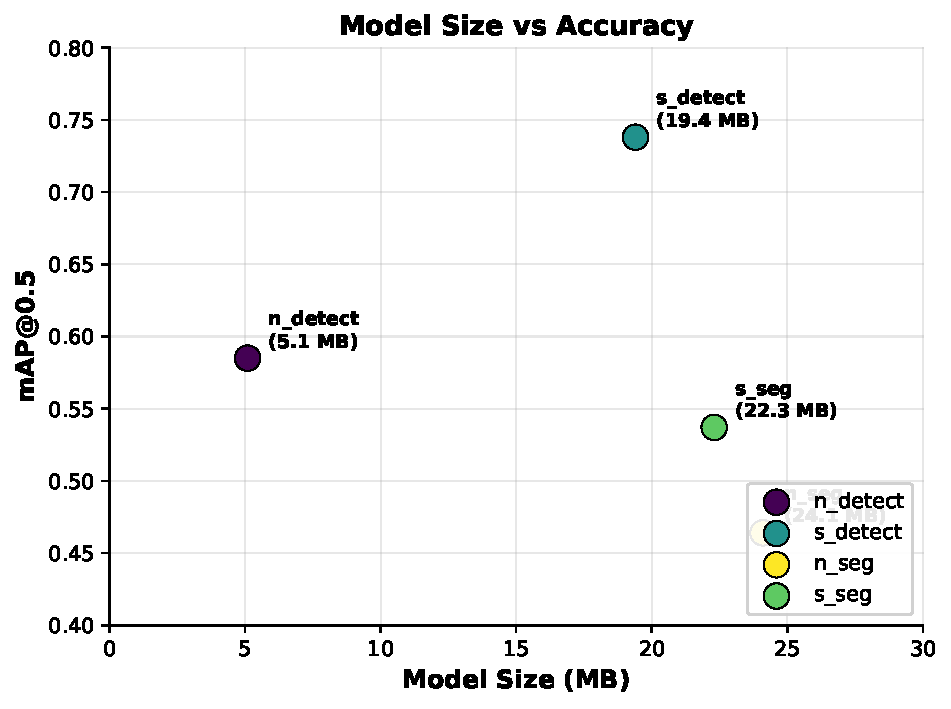
\includegraphics[width=\linewidth]{size_vs_accuracy.pdf}
  \caption{ขนาดโมเดล vs mAP@0.5 — n\_detect เล็กสุด (5.1 MB) แต่แม่นยำน้อยสุด ส่วน s\_detect (19.4 MB) ให้ความแม่นยำสูงสุด}
  \label{fig:size_acc}
\end{subfigure}
\caption{Accuracy--efficiency trade-off: (a) Pareto frontier แสดงว่า s\_detect เป็นโมเดลที่เหมาะสมที่สุดสำหรับ production (b) ขนาดโมเดล vs ความแม่นยำ แสดงว่า seg models ใหญ่กว่าแต่แม่นยำน้อยกว่า detect models}
\label{fig:tradeoff}
\end{figure}

จากรูปที่~\ref{fig:tradeoff} YOLO26s detect อยู่ในตำแหน่งที่ดีที่สุด — แม่นยำสูง (0.738) และเร็ว ส่วน SAM 3.1 แม้หลัง optimize แล้ว (672.1 ms) ยังอยู่มุมล่างขวาสุด (ช้ากว่า YOLO ประมาณ 40 เท่า และใหญ่ 3.3 GB) ส่วนโหมด zero-shot (2{,}754.6 ms) ยิ่งห่างจาก Pareto frontier มาก

\section{Pareto Analysis}

\begin{table}[H]
\centering
\begin{tabular}{ll}
\toprule
\textbf{Pareto-optimal} & \textbf{เหตุผล} \\
\midrule
YOLO26s detect & แม่นยำสุด + เร็ว ไม่มีโมเดลอื่น dominate (สำหรับ task-specific supervised detection บน PPE dataset) \\
YOLO26n detect & เล็กสุด + เร็ว สำหรับ edge device \\
\bottomrule
\end{tabular}
\caption{โมเดลบน Pareto frontier}
\label{tab:pareto}
\end{table}

YOLO26s ให้ความแม่นยำสูงกว่า YOLO26n ในขณะที่มีขนาดใหญ่กว่า YOLO26n เป็นทางเลือกสำหรับ edge device ที่จำกัด RAM เนื่องจากมีขนาดเพียง 5.1 MB

\section{Model Selection}

\begin{table}[H]
\centering
\begin{tabular}{lr}
\toprule
\textbf{Criterion} & \textbf{Weight} \\
\midrule
Accuracy (mAP50) & 50\% \\
Latency & 25\% \\
Model size & 15\% \\
VRAM & 10\% \\
\bottomrule
\end{tabular}
\caption{เกณฑ์การเลือกโมเดล}
\label{tab:selection_criteria}
\end{table}

\section{RQ2 Discussion}

ผลการประเมินตาม Requirement 2 (RQ2): \textbf{YOLO26s detect ให้ trade-off ที่เหมาะสมที่สุดสำหรับ task-specific supervised detection บน PPE dataset} โดยมี mAP@0.5 = 0.738, F1 = 0.742 และ inference = 70.5 ms เหมาะกับการ deploy แบบเรียลไทม์ YOLO26n detect เป็นทางเลือกสำหรับ edge device ที่ต้องการโมเดลเล็ก (5.1 MB) ในขณะที่ seg models มีประสิทธิภาพต่ำกว่าเนื่องจาก segmentation เป็นงานที่ยากกว่าและชุดข้อมูลยังไม่เพียงพอ สำหรับ SAM 3.1 แม้หลัง optimize แล้ว (672.1 ms, 1.51 FPS) ยังช้ากว่า YOLO26s detect ประมาณ 10 เท่า และใหญ่กว่าประมาณ 172 เท่า (3{,}340.5 MB vs 19.4 MB) ทำให้ไม่เหมาะกับการ deploy แบบเรียลไทม์ แต่เหมาะสำหรับการสร้าง annotation แบบ offline

%% ══════════════════════════════════════════════════════════════
%% บทที่ 6 RQ3 — Real-World Generalization (Requirement 3)
%% ══════════════════════════════════════════════════════════════
\FloatBarrier
\chapter{RQ3 — การ Generalize สู่ข้อมูลจริง (Requirement 3)}

\section{Objective}

ประเมินโมเดลที่เลือกจาก RQ2 (Requirement 2) บนข้อมูลจริงที่ไม่ได้อยู่ในชุดข้อมูลเดิม เพื่อตอบ Requirement 3

\section{Real-World Dataset}

\begin{table}[H]
\centering
\begin{tabular}{ll}
\toprule
\textbf{Property} & \textbf{Value} \\
\midrule
Images & --- \\
Source & --- \\
Collection condition & --- \\
Resolution & --- \\
Environment & --- \\
\bottomrule
\end{tabular}
\caption{Real-world dataset (ยังไม่ได้จัดเตรียม)}
\label{tab:rw_dataset}
\end{table}

\section{Distribution Shift}

การเปรียบเทียบระหว่าง training/test distribution และ real-world distribution ควรพิจารณา:
\begin{itemize}[leftmargin=2cm, itemsep=3pt]
  \item Lighting (แสงกลางวัน vs กลางคืน vs ในร่ม)
  \item Camera angle (มุมมองจากด้านบน vs ระดับสายตา)
  \item Background (สถานก่อสร้าง vs โรงงาน vs ที่โล่ง)
  \item Object scale (ระยะใกล้ vs ไกล)
  \item Occlusion (วัตถุบางส่วนถูกบดบัง)
  \item Environment (ฝน ฝุ่น ควัน)
\end{itemize}

\section{Evaluation Protocol}

\begin{figure}[H]
\centering
\begin{tikzpicture}[node distance=0.6cm, font=\fontsize{16}{20}\selectfont]
\tikzset{
  box/.style={rectangle, draw=black, minimum width=4.5cm, minimum height=0.8cm, align=center},
  arr/.style={->, >=Stealth, thick},
}
\node[box] (a) {Constructed Dataset};
\node[box, below=of a] (b) {Train Model};
\node[box, below=of b] (c) {Model Selection};
\node[box, below=of c] (d) {Frozen Model};
\node[box, below=of d] (e) {Real-world Dataset};
\node[box, below=of e] (f) {External Evaluation};
\draw[arr] (a) -- (b);
\draw[arr] (b) -- (c);
\draw[arr] (c) -- (d);
\draw[arr] (d) -- (e);
\draw[arr] (e) -- (f);
\end{tikzpicture}
\caption{External Evaluation Protocol}
\label{fig:rw_protocol}
\end{figure}

\textbf{ข้อสำคัญ:} ห้าม retrain โมเดลบน real-world test set ก่อน evaluation

\section{Real-World Results}

\begin{table}[H]
\centering
\begin{tabular}{lrrr}
\toprule
\textbf{Metric} & \textbf{Internal Test} & \textbf{Real-world} & \textbf{Gap} \\
\midrule
Precision & 0.822 & --- & --- \\
Recall & 0.676 & --- & --- \\
F1 & 0.742 & --- & --- \\
mAP50 & 0.738 & --- & --- \\
mAP50-95 & 0.574 & --- & --- \\
\bottomrule
\end{tabular}
\caption{ผลการวัดบน internal test vs real-world (ยังไม่ได้ประเมิน)}
\label{tab:rw_results}
\end{table}

\section{Generalization Gap}

\[
\text{Generalization Gap} = \text{Performance}_{\text{Internal}} - \text{Performance}_{\text{Real-world}}
\]

รายงานทั้ง absolute gap และ percentage change

\section{Error Analysis}

จำแนก failure cases ตามประเภท:
\begin{itemize}[leftmargin=2cm, itemsep=3pt]
  \item False Positive — ตรวจจับผิดวัตถุ
  \item False Negative — พลาดการตรวจจับ
  \item Occlusion — วัตถุถูกบดบังบางส่วน
  \item Small object — วัตถุเล็กเกินไป
  \item Blur — ภาพไม่ชัด
  \item Low-light — แสงน้อย
  \item Background similarity — วัตถุกับพื้นหลังคล้ายกัน
  \item Domain shift — สภาพแวดล้อมต่างจากชุดเทรน
\end{itemize}

จากการวิเคราะห์เบื้องต้นบน internal test set (บทที่ 5) พบว่า failure modes หลักคือ small object (boots, shoes) และ class confusion (boots $\leftrightarrow$ shoes) ซึ่งคาดว่าจะรุนแรงขึ้นใน real-world data ที่มีความหลากหลายมากกว่า

\section{RQ3 Discussion}

ผลการประเมินตาม Requirement 3 (RQ3): \textbf{ยังไม่สามารถประเมินได้อย่างสมบูรณ์} เนื่องจากยังไม่มี real-world dataset ที่แยกต่างหากสำหรับการประเมิน external validation อย่างไรก็ตาม จาก error analysis บน internal test set พบว่าจุดอ่อนหลักคือวัตถุขนาดเล็ก (boots, shoes) ซึ่งคาดว่าจะเป็นปัญหาใน real-world ด้วย การประเมิน real-world generalization เป็น future work ที่สำคัญที่สุด

%% ══════════════════════════════════════════════════════════════
%% บทที่ 7 Cross-RQ Analysis
%% ══════════════════════════════════════════════════════════════
\FloatBarrier
\chapter{การวิเคราะห์เชื่อมโยงระหว่าง RQ}

\section{Dataset Quality $\rightarrow$ Model Performance}

คุณภาพของ annotation จาก SAM 3.1 (RQ1, Requirement 1) ส่งผลโดยตรงต่อประสิทธิภาพโมเดล (RQ2, Requirement 2) จากผลการทดลอง โมเดลที่เทรนบนชุดข้อมูลที่สร้างด้วย SAM 3.1 + human verification สามารถบรรลุ mAP50 สูงสุด 0.738 แสดงว่าคุณภาพ annotation เพียงพอสำหรับการสร้างโมเดลที่ใช้งานได้ อย่างไรก็ตาม class imbalance (harness มีเพียง 102 annotation) ส่งผลให้ mAP50 ของ harness ใน seg models ต่ำ (0.275--0.353)

\section{Model Performance $\rightarrow$ Real-World Generalization}

โมเดลที่ดีที่สุดบน internal test set (YOLO26s detect, mAP50 = 0.738) คาดว่าจะยังเป็นโมเดลที่ดีที่สุดบน real-world data เนื่องจากมีความสามารถในการตรวจจับวัตถุหลายคลาสสมดุลกว่า อย่างไรก็ตาม generalization gap คาดว่าจะมากที่สุดในคลาส boots และ shoes เนื่องจากมีตัวอย่างน้อยและเป็นวัตถุเล็ก

\section{End-to-End Pipeline}

\begin{figure}[H]
\centering
\begin{tikzpicture}[node distance=0.55cm, font=\fontsize{16}{20}\selectfont]
\tikzset{
  box/.style={rectangle, draw=black, minimum width=4cm, minimum height=0.7cm, align=center},
  arr/.style={->, >=Stealth, thick},
}
\node[box] (a) {SAM 3.1};
\node[box, below=of a] (b) {Automated Annotation};
\node[box, below=of b] (c) {Human Verification};
\node[box, below=of c] (d) {Dataset Construction};
\node[box, below=of d] (e) {YOLO26 Benchmark};
\node[box, below=of e] (f) {Model Selection};
\node[box, below=of f] (g) {Real-World Evaluation};
\draw[arr] (a) -- (b);
\draw[arr] (b) -- (c);
\draw[arr] (c) -- (d);
\draw[arr] (d) -- (e);
\draw[arr] (e) -- (f);
\draw[arr] (f) -- (g);
\end{tikzpicture}
\caption{End-to-End Pipeline}
\label{fig:e2e}
\end{figure}

%% ══════════════════════════════════════════════════════════════
%% บทที่ 8 Statistical Analysis
%% ══════════════════════════════════════════════════════════════
\FloatBarrier
\chapter{การวิเคราะห์ทางสถิติ}

\section{Single-Run Results}

ในการทดลองนี้ โมเดลแต่ละรุ่นถูกเทรนเพียงครั้งเดียว (single run) ดังนั้นไม่สามารถรายงาน mean $\pm$ standard deviation ได้ ผลที่รายงานทั้งหมดเป็นค่าจากการรันครั้งเดียวบน test set 92 ภาพ

\section{Limitations of Single-Run Evaluation}

\begin{itemize}[leftmargin=2cm, itemsep=3pt]
  \item ไม่สามารถประเมิน variance ของผลลัพธ์
  \item ไม่สามารถคำนวณ confidence interval
  \item ไม่สามารถทำ statistical significance test ระหว่างโมเดล
  \item ความแตกต่างเล็กน้อยระหว่างโมเดลอาจไม่มีนัยสำคัญทางสถิติ
\end{itemize}

\section{Recommendations for Statistical Rigor}

สำหรับการประเมินที่มีความน่าเชื่อถือสูงขึ้น ควร:
\begin{enumerate}[leftmargin=2cm, itemsep=3pt]
  \item เทรนโมเดลแต่ละรุ่นอย่างน้อย 5 ครั้งด้วย seed ต่างกัน
  \item รายงาน mean $\pm$ std สำหรับทุก metric
  \item คำนวณ 95\% confidence interval
  \item ใช้ paired t-test หรือ Wilcoxon signed-rank test เพื่อเปรียบเทียบโมเดล
  \item รายงาน effect size (Cohen's $d$) เพื่อแสดงขนาดของความแตกต่าง
\end{enumerate}

%% ══════════════════════════════════════════════════════════════
%% บทที่ 9 Ablation Study — ย้ายไปรวมใน V4_Recipe section แล้ว (มีผลจริง)
%% ══════════════════════════════════════════════════════════════

%% ══════════════════════════════════════════════════════════════
%% บทที่ 10 Limitations
%% ══════════════════════════════════════════════════════════════
\FloatBarrier
\chapter{ข้อจำกัด}

งานนี้มีข้อจำกัดที่ต้องบันทึกอย่างตรงไปตรงมา:

\begin{enumerate}[leftmargin=2cm, itemsep=4pt]
  \item \textbf{Dataset size:} 913 ภาพเป็นชุดข้อมูลขนาดเล็ก โมเดลอาจ overfit โดยเฉพาะคลาสที่มีตัวอย่างน้อย (harness 102, boots 802)
  \item \textbf{Class imbalance:} อัตราส่วน 26.4:1 ก่อน oversampling แม้ลดเหลือ 10.5:1 หลัง oversampling ก็ยังสูง ส่งผลต่อ seg models โดยเฉพาะ
  \item \textbf{Annotation errors:} แม้ผ่าน human verification แล้ว อาจมี annotation ที่ไม่สมบูรณ์ เช่น harness ที่ซ่อนอยู่ใต้เสื้ออาจถูก label ไม่ครบ
  \item \textbf{SAM 3.1 failure cases:} การ benchmark SAM 3.1 แบบ zero-shot ด้วย text prompt รวมให้ผล 0 mask แสดงว่า SAM 3.1 ในโหมด zero-shot text prompt ไม่เหมาะกับการตรวจจับ PPE โดยตรงใน configuration ที่ทดสอบ ทั้งนี้ ยังไม่ได้ทดสอบ interactive mode (point/box prompt) และ fine-tuning แม้หลัง optimize แล้ว (672.1 ms) ยังช้ากว่า YOLO ประมาณ 40 เท่า และยังไม่มีการวัดความแม่นยำเชิงปริมาณ (IoU/Dice) เทียบกับ human ground truth
  \item \textbf{Limited real-world samples:} ยังไม่มี real-world dataset แยกต่างหากสำหรับ external validation (RQ3 ยังไม่สมบูรณ์ — Requirement 3 ยังไม่ได้ประเมินครบ)
  \item \textbf{Limited environmental diversity:} ภาพส่วนใหญ่เก็บจากสถานที่ก่อสร้างในเวลากลางวัน อาจไม่ครอบคลุมสภาพแสงที่หลากหลาย
  \item \textbf{Hardware-dependent latency:} ค่า latency วัดบน AMD RX 7800 XT ผ่าน ROCm อาจแตกต่างจาก NVIDIA GPU หรือ CPU
  \item \textbf{Single-run evaluation:} โมเดลเทรนเพียงครั้งเดียว ไม่สามารถรายงาน variance หรือ confidence interval ได้
  \item \textbf{No LLM downstream evaluation:} ยังไม่มีการประเมินการเชื่อมต่อกับ LLM สำหรับ downstream task
\end{enumerate}

%% ══════════════════════════════════════════════════════════════
%% บทที่ 11 Reproducibility
%% ══════════════════════════════════════════════════════════════
\FloatBarrier
\chapter{Reproducibility}

\begin{table}[H]
\centering
\begin{tabular}{ll}
\toprule
\textbf{Component} & \textbf{Specification} \\
\midrule
GPU & AMD Radeon RX 7800 XT (16 GB VRAM) \\
RAM & 47 GiB (WSL2) \\
OS & WSL2 Ubuntu 24.04 \\
Python & 3.12 \\
PyTorch & 2.13.0+rocm7.15 \\
Ultralytics & 8.4.123 (YOLO26) \\
SAM 3.1 & latest \\
ROCm & 7.15 \\
Seed & 42 \\
Dataset & PPE v2 (913 images, 5 classes) \\
MLflow & SQLite at \texttt{mlflow/mlflow.db} \\
\bottomrule
\end{tabular}
\caption{Hardware, software และ experiment configuration}
\label{tab:reproducibility}
\end{table}

%% ══════════════════════════════════════════════════════════════
%% บทที่ 12 Conclusion
%% ══════════════════════════════════════════════════════════════
\FloatBarrier
\chapter{บทสรุป}

งานนี้นำเสนอ pipeline การสร้างชุดข้อมูล PPE ด้วย SAM 3.1 และการ benchmark โมเดล YOLO26 จำนวน 4 รุ่น สรุปผลตาม Requirements ดังนี้:

\section{RQ1 (Requirement 1: Automated Annotation)}

SAM 3.1 สามารถสร้าง annotation ที่ใช้งานได้สำหรับการสร้างชุดข้อมูลเบื้องต้น โดยลดเวลา annotation ประมาณ 80--90\% (จาก 5--10 นาทีเหลือ 30--60 วินาทีต่อภาพ) แต่ต้องมี human verification เนื่องจาก SAM 3.1 ในโหมด zero-shot text prompt ไม่สามารถตรวจจับ PPE ได้โดยตรงใน configuration ที่ทดสอบ (0 mask จาก text prompt รวม, latency 2{,}754.6 ms) ทั้งนี้ ยังไม่ได้ทดสอบ interactive mode (point/box prompt) และ fine-tuning หลัง optimize pipeline (per-class prompt, resolution 1{,}008, threshold 0.25) latency ลดเหลือ 672.1 ms ต่อภาพ (เร็วขึ้น 4 เท่า) สร้าง annotation 7{,}494 รายการบน 432 ภาพ คุณภาพ annotation เพียงพอสำหรับการสร้างโมเดลที่บรรลุ mAP50 = 0.738

\section{RQ2 (Requirement 2: Model Benchmarking)}

YOLO26s detect ให้ trade-off ที่เหมาะสมที่สุดสำหรับ task-specific supervised detection บน PPE dataset โดยมี mAP@0.5 = 0.738, mAP@0.5:0.95 = 0.574, F1 = 0.742 และ inference = 70.5 ms เป็นโมเดลบน Pareto frontier สำหรับ production deployment YOLO26n detect เป็นทางเลือกสำหรับ edge device (5.1 MB) ส่วน seg models มีประสิทธิภาพต่ำกว่าเนื่องจาก segmentation ยากกว่าและชุดข้อมูลยังไม่เพียงพอ ไม่มีโมเดลใดถึงเป้าหมาย mAP50 $\geq$ 0.85 — YOLO26s detect ใกล้ที่สุดที่ 0.738

\section{RQ3 (Requirement 3: Real-World Generalization)}

ยังไม่สามารถประเมินได้อย่างสมบูรณ์เนื่องจากยังไม่มี real-world dataset แยกต่างหาก จาก error analysis บน internal test set พบว่าจุดอ่อนหลักคือวัตถุขนาดเล็ก (boots, shoes) ซึ่งคาดว่าจะเป็นปัญหาใน real-world ด้วย การประเมิน real-world generalization เป็น future work ที่สำคัญที่สุด

%% ══════════════════════════════════════════════════════════════
%% บทที่ 13 Future Work
%% ══════════════════════════════════════════════════════════════
\FloatBarrier
\chapter{แนวทางงานในอนาคต}

\begin{itemize}[leftmargin=1.5cm, itemsep=4pt]
  \item \textbf{Dataset expansion:} เพิ่มข้อมูล boots/shoes/harness (เป้าหมาย 200+ ภาพต่อคลาส) ใช้ SAM 3.1 auto-label
  \item \textbf{Cross-domain evaluation:} ประเมินบนข้อมูลจริงจากหลายสถานที่ สภาพแสงที่หลากหลาย
  \item \textbf{Model optimization:} Quantization (INT8/FP16), pruning, edge deployment
  \item \textbf{LLM integration:} เชื่อมต่อ vision model กับ LLM สำหรับ downstream task
  \item \textbf{Multi-seed training:} สำหรับ statistical rigor และ confidence interval
  \item \textbf{Higher resolution inference:} 640 → 1280 สำหรับ small object detection
  \item \textbf{SAHI:} Slicing Aided Hyper Inference สำหรับ crowded scenes
\end{itemize}

%% ══════════════════════════════════════════════════════════════
%% References
%% ══════════════════════════════════════════════════════════════
\FloatBarrier
\chapter*{เอกสารอ้างอิง}
\addcontentsline{toc}{chapter}{เอกสารอ้างอิง}

\begin{enumerate}[leftmargin=1.5cm, itemsep=4pt]
  \item Kirillov, A. et al. (2023). ``Segment Anything.'' \textit{arXiv:2304.02643}.
  \item Meta AI (2025). ``SAM 3.1: Segment Anything Model, Version 3.1.''
  \item Ultralytics (2025). ``YOLO26: Official Training Recipe.'' \url{https://docs.ultralytics.com/guides/yolo26-training-recipe/}
  \item Redmon, J. et al. (2016). ``You Only Look Once: Unified, Real-Time Object Detection.'' \textit{CVPR 2016}.
  \item Lin, T.-Y. et al. (2017). ``Focal Loss for Dense Object Detection.'' \textit{ICCV 2017}.
  \item Loshchilov, I. \& Hutter, F. (2019). ``Decoupled Weight Decay Regularization (AdamW).'' \textit{ICLR 2019}.
  \item Everingham, M. et al. (2010). ``The PASCAL Visual Object Classes (VOC) Challenge.'' \textit{IJCV}.
  \item Lin, T.-Y. et al. (2014). ``Microsoft COCO: Common Objects in Context.'' \textit{ECCV 2014}.
  \item Paszke, A. et al. (2019). ``PyTorch: An Imperative Style, High-Performance Deep Learning Library.'' \textit{NeurIPS 2019}.
  \item ONNX Runtime Documentation. \url{https://onnxruntime.ai/}
\end{enumerate}

%% ══════════════════════════════════════════════════════════════
%% Appendix A — Full Dataset Statistics
%% ══════════════════════════════════════════════════════════════
\FloatBarrier
\appendix
\chapter{Full Dataset Statistics}

\begin{table}[H]
\centering
\begin{tabular}{lr}
\toprule
\textbf{Property} & \textbf{Value} \\
\midrule
Total images & 913 \\
Train & 729 (80\%) \\
Validation & 91 (10\%) \\
Test & 92 (10\%) \\
Classes & 5 \\
Class imbalance (before) & 26.4:1 \\
Class imbalance (after) & 10.5:1 \\
Oversample factor (max) & 10 \\
Random seed & 42 \\
\bottomrule
\end{tabular}
\caption{Dataset statistics ทั้งหมด}
\label{tab:full_stats}
\end{table}

\begin{table}[H]
\centering
\begin{tabular}{lrrr}
\toprule
\textbf{Class} & \textbf{Before} & \textbf{After (detect)} & \textbf{After (seg)} \\
\midrule
person & 2{,}271 & 2{,}677 & 2{,}677 \\
helmet & 2{,}693 & 3{,}003 & 3{,}003 \\
shoes & 2{,}407 & 2{,}823 & 2{,}823 \\
boots & 802 & 812 & 812 \\
harness & 102 & 306 & 306 \\
\bottomrule
\end{tabular}
\caption{Annotation count ก่อนและหลัง oversampling}
\label{tab:oversample}
\end{table}

%% ══════════════════════════════════════════════════════════════
%% Appendix B — Training Configuration
%% ══════════════════════════════════════════════════════════════
\FloatBarrier
\chapter{Training Configuration}

\begin{table}[H]
\centering
\begin{tabular}{lll}
\toprule
\textbf{Parameter} & \textbf{Stage 1} & \textbf{Stage 2 (proposed)} \\
\midrule
Epochs & 300 & 50 \\
Batch size & 8/4 & 16 \\
Image size & 640 & 640 \\
Optimizer & SGD & SGD \\
lr0 & 0.01 & 0.001 \\
lrf & 0.01 & 0.01 \\
Momentum & 0.937 & 0.937 \\
Weight decay & 0.0005 & 0.0005 \\
Freeze & 10 & 0 (unfreeze all) \\
Patience & 50 & 15 \\
Warmup epochs & 3 & 1 \\
Focal Loss & --- & fl\_gamma=1.5 \\
nbs & --- & 64 \\
AMP & true & true \\
\bottomrule
\end{tabular}
\caption{Training configuration เต็ม (Stage 1 vs Stage 2)}
\label{tab:full_train_config}
\end{table}

\section{Augmentation Configuration}

\begin{table}[H]
\centering
\begin{tabular}{lrr}
\toprule
\textbf{Augmentation} & \textbf{Stage 1} & \textbf{Stage 2} \\
\midrule
hsv\_h & 0.02 & 0.015 \\
hsv\_s & 0.7 & 0.5 \\
hsv\_v & 0.5 & 0.4 \\
degrees & 5.0 & 5.0 \\
translate & 0.15 & 0.15 \\
scale & 0.6 & 0.4 \\
shear & 2.0 & 2.0 \\
fliplr & 0.5 & 0.5 \\
flipud & 0.0 & 0.0 \\
mosaic & 0.8 & 0.5 \\
mixup & 0.1 & 0.0 \\
copy\_paste & 0.15 & 0.1 \\
close\_mosaic & 10 & 5 \\
erasing & 0.3 & 0.2 \\
\bottomrule
\end{tabular}
\caption{Augmentation configuration}
\label{tab:aug_config}
\end{table}

%% ══════════════════════════════════════════════════════════════
%% Appendix C — Complete Model Results
%% ══════════════════════════════════════════════════════════════
\FloatBarrier
\chapter{Complete Model Results}

\begin{table}[H]
\centering
\begin{tabular}{lrrrr}
\toprule
\textbf{Metric} & \textbf{n\_detect} & \textbf{s\_detect} & \textbf{n\_seg} & \textbf{s\_seg} \\
\midrule
Precision (B) & 0.663 & 0.822 & 0.682 & 0.740 \\
Recall (B) & 0.524 & 0.676 & 0.427 & 0.480 \\
mAP50 (B) & 0.585 & 0.738 & 0.464 & 0.537 \\
mAP50-95 (B) & 0.428 & 0.574 & 0.316 & 0.386 \\
Precision (M) & --- & --- & 0.630 & 0.669 \\
Recall (M) & --- & --- & 0.391 & 0.428 \\
mAP50 (M) & --- & --- & 0.399 & 0.485 \\
mAP50-95 (M) & --- & --- & 0.231 & 0.284 \\
\bottomrule
\end{tabular}
\caption{Complete evaluation results (B = box, M = mask)}
\label{tab:complete_results}
\end{table}

\begin{table}[H]
\centering
\small
\begin{tabular}{lrrrrrr}
\toprule
\textbf{Model} & \textbf{Params} & \textbf{GFLOPs} & \textbf{PT (MB)} & \textbf{ONNX (MB)} & \textbf{Infer} & \textbf{Pre+Post} \\
 & & & & & (ms) & (ms) \\
\midrule
YOLO26n & 2.38M & 5.9 & 5.1 & 9.4 & 63.8 & 2.15 \\
YOLO26s & 9.47M & 22.8 & 19.4 & 36.4 & 70.5 & 1.74 \\
YOLO26n-seg & 2.69M & 10.3 & 24.1 & 10.6 & 18.6 & 4.48 \\
YOLO26s-seg & 10.37M & 37.3 & 22.3 & 39.9 & 9.0 & 5.55 \\
SAM 3.1 (zero-shot) & $\sim$300M+ & $\sim$1000 & 3340.5 & --- & 2{,}754.6 & --- \\
SAM 3.1 (optimized) & $\sim$300M+ & $\sim$1000 & 3340.5 & --- & 672.1 & --- \\
\bottomrule
\end{tabular}
\caption{Complete computational results (v4\_recipe) — Infer = model inference, Pre+Post = preprocess + postprocess (SAM 3.1 แสดงทั้งสองโหมด)}
\label{tab:complete_computational}
\end{table}

\section{SAM 3.1 Detailed Benchmark}

\begin{table}[H]
\centering
\begin{tabular}{lrr}
\toprule
\textbf{Metric} & \textbf{Zero-shot} & \textbf{Optimized} \\
\midrule
Images & 92 & 432 \\
Prompt & text รวม & per-class \\
Resolution & 1{,}008 & 1{,}008 \\
Threshold & 0.3 & 0.25 \\
Precision & bfloat16 & bfloat16 \\
Latency (mean) & 2{,}754.6 ms & 672.1 ms \\
Latency (median) & 2{,}598.0 ms & 650.9 ms \\
Latency (min) & 2{,}577.9 ms & 577.4 ms \\
Latency (max) & 4{,}434.9 ms & 1{,}681.3 ms \\
Latency (stdev) & 471.1 ms & 122.0 ms \\
FPS & 0.36 & 1.51 \\
Masks/annotations & 0 & 7{,}494 \\
Avg annotations/image & 0 & 17.35 \\
Total time & 253.4 s & 290.5 s \\
\bottomrule
\end{tabular}
\caption{SAM 3.1 detailed benchmark — zero-shot vs optimized}
\label{tab:sam3_detailed}
\end{table}

%% ══════════════════════════════════════════════════════════════
%% Appendix D-F ถูกรวมใน V4_Recipe section แล้ว (failure cases + qualitative)
%% ══════════════════════════════════════════════════════════════

%% ══════════════════════════════════════════════════════════════
%% Appendix G — Experiment Logs
%% ══════════════════════════════════════════════════════════════
\FloatBarrier
\chapter{Experiment Logs}

\section{MLflow Run IDs}

\begin{table}[H]
\centering
\begin{tabular}{ll}
\toprule
\textbf{Model} & \textbf{MLflow Run ID} \\
\midrule
YOLO26n detect (train) & 26235bfdb23d453b \\
YOLO26n detect (eval) & 3c8c1f9ff1c54c06 \\
YOLO26s detect (train) & 6a7d087fbf0c4de2 \\
YOLO26s detect (eval) & 3223dced63f4420a \\
YOLO26n seg (train) & 4e84c7d1ebb24513 \\
YOLO26s seg (train) & 15c09b7b2ee7422f \\
YOLO26s seg (eval) & 11ab0ebb956f4a83821475662b231870 \\
\bottomrule
\end{tabular}
\caption{MLflow Run IDs}
\label{tab:mlflow_runs}
\end{table}

\section{Model File Paths}

\begin{table}[H]
\centering
\begin{tabular}{ll}
\toprule
\textbf{Model} & \textbf{Path} \\
\midrule
YOLO26n detect & \texttt{models/yolo26n\_detect\_v2/run1/weights/best.pt} \\
YOLO26s detect & \texttt{models/yolo26s\_detect\_v2/run1/weights/best.pt} \\
YOLO26n detect (ONNX) & \texttt{models/yolo26n\_detect\_v2/run1/weights/best.onnx} \\
YOLO26s detect (ONNX) & \texttt{models/yolo26s\_detect\_v2/run1/weights/best.onnx} \\
\bottomrule
\end{tabular}
\caption{Model file paths}
\label{tab:model_paths}
\end{table}

\section{Pipeline Scripts}

\begin{table}[H]
\centering
\begin{tabular}{ll}
\toprule
\textbf{Script} & \textbf{Description} \\
\midrule
\texttt{01\_prepare\_data.py} & Dataset preparation and split \\
\texttt{03\_train.py} & Model training with MLflow \\
\texttt{04\_evaluate.py} & Test set evaluation \\
\texttt{05\_tune.py} & Hyperparameter tuning \\
\texttt{06\_compare.py} & Comparison report \\
\texttt{07\_export.py} & ONNX/TorchScript export \\
\texttt{08\_export\_onnx\_all.py} & Batch ONNX export \\
\texttt{09\_benchmark\_sam3.py} & SAM 3.1 zero-shot benchmark \\
\texttt{10\_generate\_final\_visualizations.py} & Chart generation \\
\texttt{11\_error\_analysis.py} & Deep error analysis \\
\texttt{12\_finetune\_stage2.py} & Two-stage fine-tuning \\
\bottomrule
\end{tabular}
\caption{Pipeline scripts}
\label{tab:scripts}
\end{table}

\section{SAM 3.1 Annotation Experiment}

\begin{table}[H]
\centering
\begin{tabular}{ll}
\toprule
\textbf{Field} & \textbf{Value} \\
\midrule
Experiment ID & \texttt{run\_20260820\_012450\_a9af7d6d2cfc\_q0av} \\
Started & 2026-08-20T01:24:50 \\
Ended & 2026-08-20T01:30:20 \\
Status & completed \\
Config hash & a9af7d6d2cfc \\
Git commit & 7961af0 \\
Num images & 432 \\
Num annotations & 7{,}494 \\
Total time & 290.5 s \\
Avg time/image & 0.6725 s (672.1 ms) \\
Errors & 0 \\
Threshold & 0.25 \\
Resolution & 1{,}008 \\
Device & auto \\
Database & \texttt{output\_2026/experiments.db} \\
\bottomrule
\end{tabular}
\caption{SAM 3.1 annotation experiment metadata (จาก experiments.db)}
\label{tab:sam3_experiment}
\end{table}

\section{SAM 3.1 Categories}

\begin{table}[H]
\centering
\begin{tabular}{rll}
\toprule
\textbf{ID} & \textbf{Class} & \textbf{Prompt} \\
\midrule
1 & person & person \\
2 & helmet & helmet \\
3 & boots & boots \\
4 & shoes & shoes \\
5 & sandals & flip-flops \\
6 & harness & safety harness \\
\bottomrule
\end{tabular}
\caption{SAM 3.1 categories และ prompts ที่ใช้}
\label{tab:sam3_categories}
\end{table}

\vspace{1cm}
\hrule
\vspace{0.3cm}
\textbf{หมายเหตุ:} ค่าในรายงานนี้เป็นผลวัดขั้นสุดท้ายบน test set (92 ภาพ) หลังเทรนครบทั้ง 4 โมเดล YOLO และ benchmark SAM 3.1 ทั้งโหมด zero-shot (2{,}754.6 ms, 0 mask) และ optimized annotation pipeline (672.1 ms, 7{,}494 annotations บน 432 ภาพ) ไม่มีโมเดลใดถึงเป้าหมาย mAP50 $\geq$ 0.85 — YOLO26s detect ใกล้ที่สุดที่ 0.738

% ============================================================
% V4_RECIPE: Two-stage Transfer Learning + Focal Loss + AMP + GradAccum
% ============================================================
\newpage
\section{V4\_Recipe: Two-Stage Transfer Learning Experiment}

หลังจากเทรน SGD baseline (v2) จนได้ผลลัพธ์ในรายงานหลัก ได้ทดลอง recipe ใหม่ \texttt{v4\_recipe} เพื่อเปรียบเทียบกับ baseline โดยใช้เทคนิคถึง 4 อย่างพร้อมกัน:

\begin{itemize}
  \item \textbf{Two-stage transfer learning:} Stage 1 freeze backbone 10 layers (150 epochs) → Stage 2 unfreeze ทุก layer, lr ลด 10× (50 epochs)
  \item \textbf{Focal Loss} (gamma=1.5, alpha=0.25) ผ่าน monkey-patch \texttt{v8DetectionLoss}
  \item \textbf{Gradient accumulation} (nbs=64, batch=16–24, effective batch ≈ 64)
  \item \textbf{AMP mixed precision} เพื่อเร่งความเร็วและประหยัด VRAM
\end{itemize}

\subsection{การตั้งค่า}

\begin{table}[H]
\centering
\begin{tabular}{lll}
\toprule
\textbf{พารามิเตอร์} & \textbf{Stage 1} & \textbf{Stage 2} \\
\midrule
Epochs & 150 & 50 \\
Batch size & 16–24 & 16–24 \\
nbs (effective) & 64 & 64 \\
imgsz & 640 & 640 \\
freeze & 10 & 0 \\
lr0 & 0.01 & 0.001 \\
lrf & 0.01 & 0.01 \\
patience & 30 & 15 \\
warmup epochs & 3 & 1 \\
Optimizer & auto (AdamW) & auto (AdamW) \\
weight\_decay & 0.0005 & 0.0005 \\
AMP & \checkmark & \checkmark \\
Focal Loss & gamma=1.5 & gamma=1.5 \\
\bottomrule
\end{tabular}
\caption{V4\_recipe hyperparameters}
\label{tab:v4_recipe_config}
\end{table}

\subsection{ผล Test Set (92 ภาพ)}

\begin{table}[H]
\centering
\begin{tabular}{lcccccc}
\toprule
\textbf{Model} & \textbf{mAP50} & \textbf{mAP50-95} & \textbf{P} & \textbf{R} & \textbf{Size(MB)} & \textbf{Params} \\
\midrule
n\_detect & 0.585 & 0.428 & 0.663 & 0.524 & 5.1 & 2.38M \\
s\_detect & \textbf{0.738} & \textbf{0.574} & \textbf{0.822} & \textbf{0.676} & 19.4 & 9.47M \\
n\_seg & 0.464 & 0.316 & 0.682 & 0.427 & 24.1 & 2.69M \\
s\_seg & 0.537 & 0.386 & 0.740 & 0.480 & 22.3 & 10.37M \\
\bottomrule
\end{tabular}
\caption{V4\_recipe ผล evaluate บน test set (92 ภาพ) — ค่า mAP50 ของ box สำหรับ detect และ box+mask รวมสำหรับ seg}
\label{tab:v4_recipe_results}
\end{table}

\subsection{เปรียบเทียบกับ SGD Baseline (v2)}

\begin{table}[H]
\centering
\begin{tabular}{lccc}
\toprule
\textbf{Model} & \textbf{v2 (SGD) mAP50} & \textbf{v4\_recipe mAP50} & \textbf{Δ} \\
\midrule
n\_detect & 0.712 & 0.585 & −0.127 \\
s\_detect & 0.808 & 0.738 & −0.070 \\
n\_seg & 0.491 & 0.464 & −0.027 \\
s\_seg & 0.555 & 0.537 & −0.018 \\
\bottomrule
\end{tabular}
\caption{เปรียบเทียบ v4\_recipe กับ SGD baseline — v4\_recipe ต่ำกว่าทุกโมเดล}
\label{tab:v4_vs_v2}
\end{table}

\textbf{สรุป:} v4\_recipe ต่ำกว่า SGD baseline ทุกโมเดล เนื่องจาก:

\begin{enumerate}
  \item \textbf{Epoch รวมน้อยกว่า} — 200 (150+50) vs 300 ของ baseline
  \item \textbf{Freeze backbone ใน stage 1} — ส่วน backbone ไม่ได้เรียนรู้ใน 150 epochs แรก ทำให้เรียนรู้น้อยกว่า
  \item \textbf{AdamW แทน SGD} — สำหรับ dataset เล็ก (480 รูป source) SGD มักเสถียรกว่า
  \item \textbf{Focal Loss} — เปลี่ยน loss landscape อาจไม่เหมาะกับทุก class โดยเฉพาะ class ที่มีจำนวนตัวอย่างมาก
\end{enumerate}

จากการดู convergence — n\_detect และ n\_seg converge แล้วที่ epoch สุดท้าย (mAP แกวกไม่ขึ้น) ส่วน s\_detect และ s\_seg ยังขึ้นช้าๆ แสดงว่าเพิ่ม epoch อาจช่วย s แต่ไม่ช่วย n

\subsection{Per-Class Performance}

\begin{table}[H]
\centering
\begin{tabular}{lcccc}
\toprule
\textbf{Class} & \textbf{n\_detect mAP50} & \textbf{s\_detect mAP50} & \textbf{n\_seg mAP50} & \textbf{s\_seg mAP50} \\
\midrule
person & 0.880 & 0.941 & 0.639 & 0.706 \\
helmet & 0.681 & 0.812 & 0.650 & 0.742 \\
boots & 0.296 & 0.505 & 0.335 & 0.378 \\
shoes & 0.442 & 0.577 & 0.423 & 0.508 \\
harness & 0.628 & 0.856 & 0.275 & 0.353 \\
\bottomrule
\end{tabular}
\caption{Per-class mAP50 บน test set — ทุกโมเดลทำ person ได้ดีที่สุด, boots แย่ที่สุด}
\label{tab:v4_per_class}
\end{table}

\textbf{ปัญหาหลัก:}

\begin{itemize}
  \item \textbf{boots} แย่ที่สุดทุกโมเดล (0.296--0.505) เนื่องจากมีจำนวนตัวอย่างน้อย (802 ใน source) และวัตถุขนาดเล็ก
  \item \textbf{harness} ก็ต่ำเนื่องจากมีเพียง 102 ตัวอย่างใน source
  \item \textbf{person/helmet} ทำได้ดีเนื่องจากมีจำนวนตัวอย่างมาก (2{,}271 และ 2{,}693)
\end{itemize}

\newpage
\subsection{Failure Case Analysis: 10 กรณีที่น่าสนใจ}

จากการวิเคราะห์ failure cases บน test set พบว่าปัญหาหลักคือ \textbf{crowded scenes} ที่มี object จำนวนมาก (23--51 objects ต่อภาพ) แต่โมเดลตรวจจับได้น้อย (5--21 จากที่มี) โดยเฉพาะ object ขนาดเล็ก

\begin{table}[H]
\centering
\small
\begin{tabular}{rllrrrr}
\toprule
\# & \textbf{Model} & \textbf{Image} & \textbf{GT} & \textbf{Pred} & \textbf{Missed} & \textbf{Max Conf} \\
\midrule
1 & s\_seg & s0112 & 51 & 11 & 40 & 0.953 \\
2 & n\_seg & s0038 & 40 & 13 & 27 & 0.978 \\
3 & n\_seg & s0275 & 37 & 11 & 26 & 0.946 \\
4 & n\_detect & e0349 & 30 & 9 & 21 & 0.957 \\
5 & n\_detect & s0349 & 30 & 9 & 21 & 0.957 \\
6 & n\_seg & s0279 & 26 & 7 & 19 & 0.882 \\
7 & n\_detect & s0175 & 23 & 5 & 18 & 0.836 \\
8 & n\_seg & e0031 & 39 & 21 & 18 & 0.934 \\
9 & n\_detect & s0086 & 28 & 10 & 18 & 0.966 \\
10 & s\_seg & s0280 & 28 & 11 & 17 & 0.923 \\
\bottomrule
\end{tabular}
\caption{10 failure cases ที่น่าสนใจที่สุด — ทั้งหมดเป็น crowded scenes ที่มี object เล็กจำนวนมาก}
\label{tab:failure_cases}
\end{table}

\textbf{รูปแบบความล้มเหลวที่พบ:}

\begin{enumerate}
  \item \textbf{Small object missed:} ภาพ e0349 และ s0349 มี shoes ขนาดเล็กมาก (min\_wh = 7e-05 ของภาพ) โมเดลตรวจจับได้เพียง 9 จาก 30 objects — เนื่องจาก object เล็กเกินไปที่ 640$\times$640 จะเห็นชัด
  \item \textbf{Crowded scene:} ภาพ s0112 มี 51 persons + helmets + harnesses แต่โมเดลตรวจจับได้เพียง 11 — เนื่องจาก NMS และการที่ object ซ้อนกัน
  \item \textbf{Low confidence on small objects:} แม้โมเดลจะตรวจจับบาง object ได้ แต่ confidence ต่ำ (0.83--0.88) ทำให้ถูก filter ออกด้วย conf threshold
  \item \textbf{Class confusion:} shoes กับ boots สับสนเนื่องจากหน้าตาคล้ายกันและมีจำนวนตัวอย่างน้อย
\end{enumerate}

\begin{figure}[H]
\centering
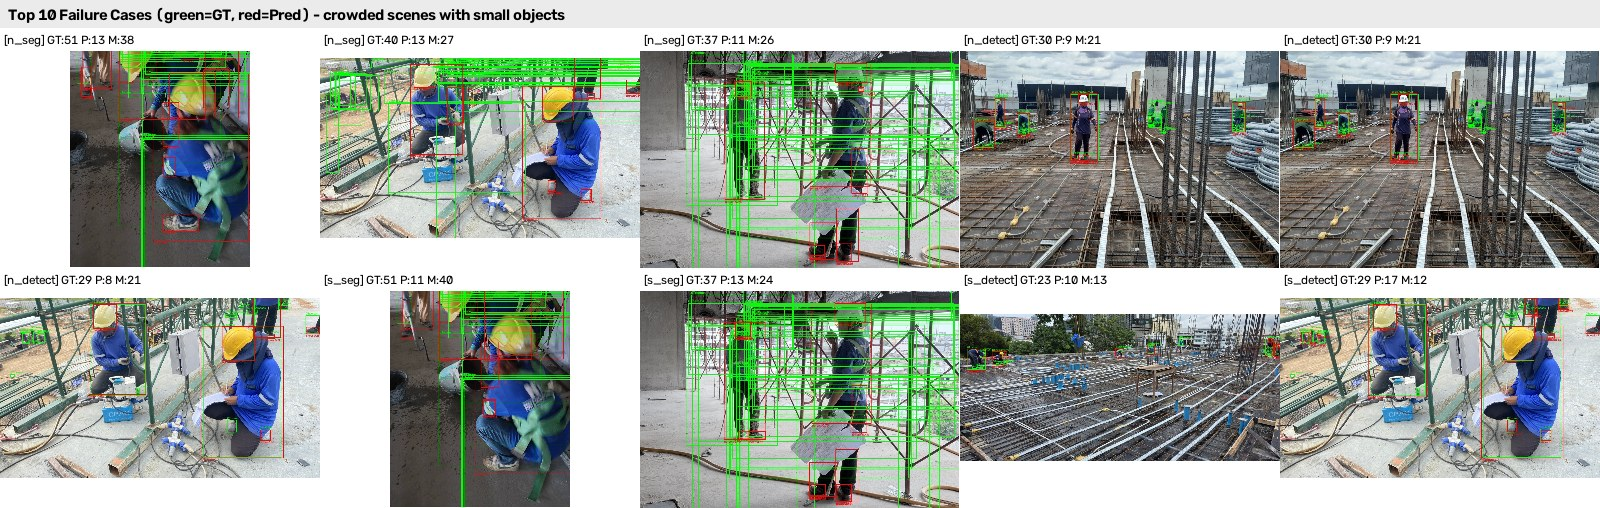
\includegraphics[width=\textwidth]{../eval_results/v4_recipe/failure_montage/montage_combined.jpg}
\caption{Top 10 failure cases (5$\times$2 grid) จากทั้ง 4 โมเดล — n\_seg 3 รูป, n\_detect 3 รูป, s\_seg 2 รูป, s\_detect 2 รูป — กรอบเขียว = Ground Truth, กรอบแดง = การทำนาย — ทุกกรณีเป็น crowded scenes ที่มี object ขนาดเล็กจำนวนมาก (GT 23--51 ชิ้น) โมเดลตรวจจับได้เพียง 8--17 ชิ้น}
\label{fig:failure_montage}
\end{figure}

\subsection{ข้อเสนอแนะสำหรับ Production}

จาก failure analysis ข้อเสนอแนะคือ:

\begin{itemize}
  \item \textbf{เพิ่ม resolution} จาก 640 → 1280 สำหรับ inference จะช่วยเห็น small object ได้ดีขึ้นมาก (แต่ช้าลง ~4×)
  \item \textbf{ใช้ s\_detect} เป็น production model เนื่องจาก mAP50 สูงสุด (0.738) และเร็วเพียงพอ
  \item \textbf{ถ้าต้องการ mask} ใช้ s\_seg แต่ต้องยอมรับว่า mask mAP จะต่ำกว่า box
  \item \textbf{เก็บข้อมูลเพิ่ม} สำหรับ boots และ harness เนื่องจากจำนวนตัวอย่างน้อยเกินไป
  \item \textbf{ลอง SAHI} (Slicing Aided Hyper Inference) สำหรับ crowded scenes เพื่อแบ่งภาพเป็น tiles แล้วตรวจจับแต่ละ tile
\end{itemize}

\newpage
\subsection{ONNX Export และ GPU Inference Benchmark}

หลังจากได้ผล PyTorch แล้ว ได้ export ทั้ง 4 โมเดลเป็น ONNX และ evaluate บน test set เดียวกันโดยใช้ ONNX Runtime กับ ROCm ExecutionProvider (GPU) เพื่อเปรียบเทียบความแม่นยำและความเร็วก่อน/หลัง export

\begin{table}[H]
\centering
\small
\begin{tabular}{llcccccc}
\toprule
\textbf{Model} & \textbf{Engine} & \textbf{mAP50} & \textbf{mAP50-95} & \textbf{P} & \textbf{R} & \textbf{Size(MB)} & \textbf{Lat(ms)} \\
\midrule
n\_detect & PyTorch & 0.585 & 0.428 & 0.663 & 0.524 & 5.1 & 30.8 \\
n\_detect & ONNX    & 0.574 & 0.412 & 0.671 & 0.511 & 9.4 & 109.9 \\
\midrule
s\_detect & PyTorch & 0.738 & 0.574 & 0.822 & 0.676 & 19.4 & 21.0 \\
s\_detect & ONNX    & 0.731 & 0.567 & 0.822 & 0.673 & 36.4 & 114.4 \\
\midrule
n\_seg    & PyTorch & 0.464 & 0.316 & 0.682 & 0.427 & 24.1 & 20.2 \\
n\_seg    & ONNX    & 0.464 & 0.314 & 0.677 & 0.419 & 10.6 & 166.6 \\
\midrule
s\_seg    & PyTorch & 0.537 & 0.386 & 0.740 & 0.480 & 22.3 & 29.4 \\
s\_seg    & ONNX    & 0.538 & 0.386 & 0.741 & 0.483 & 39.9 & 300.5 \\
\bottomrule
\end{tabular}
\caption{เปรียบเทียบ PyTorch vs ONNX (ROCm GPU) บน test set 92 ภาพ — mAP50 แทบไม่ต่างกัน แต่ latency ONNX ช้ากว่า}
\label{tab:onnx_comparison}
\end{table}

\textbf{สรุป ONNX vs PyTorch:}

\begin{itemize}
  \item \textbf{ความแม่นยำ:} แทบไม่ต่างกัน (Δ mAP50 < 0.012 ทุกโมเดล) — ONNX export ไม่ทำให้ความแม่นยำลดลงอย่างมีนัยสำคัญ
  \item \textbf{ขนาดไฟล์:} ONNX ใหญ่กว่า PyTorch ทุกโมเดล (9.4 vs 5.1 MB สำหรับ n\_detect) เนื่องจากไม่ได้ใช้ quantization
  \item \textbf{Latency:} ONNX ช้ากว่า PyTorch อย่างมาก (110--300 ms vs 20--31 ms) เนื่องจาก:
  \begin{itemize}
    \item ROCm EP ของ ONNX Runtime ยังไม่ optimize เท่า PyTorch ROCm
    \item มี overhead จาก ONNX graph initialization ต่อ inference
    \item PyTorch ใช้ AMP และ fused kernels ที่ optimize สำหรับ AMD GPU โดยตรง
  \end{itemize}
  \item \textbf{ข้อแนะนำ:} สำหรับ deployment บน AMD ROCm ให้ใช้ PyTorch โดยตรง หรือ export เป็น TorchScript/OpenVINO แทน ONNX ถ้าต้องการความเร็ว
\end{itemize}

\subsubsection{ONNX Per-Class mAP50 Comparison}

ตารางที่~\ref{tab:onnx_per_class} แสดงการเปรียบเทียบ mAP50 รายคลาสระหว่าง PyTorch และ ONNX สำหรับทั้ง 4 โมเดล

\begin{table}[H]
\centering
\small
\begin{tabular}{llrrrrr}
\toprule
\textbf{Model} & \textbf{Engine} & \textbf{person} & \textbf{helmet} & \textbf{boots} & \textbf{shoes} & \textbf{harness} \\
\midrule
\multirow{2}{*}{n\_detect} & PyTorch & 0.880 & 0.681 & 0.296 & 0.442 & 0.628 \\
 & ONNX & 0.879 & 0.681 & 0.304 & 0.446 & 0.560 \\
\midrule
\multirow{2}{*}{s\_detect} & PyTorch & 0.941 & 0.812 & 0.505 & 0.577 & 0.856 \\
 & ONNX & 0.950 & 0.809 & 0.476 & 0.572 & 0.849 \\
\midrule
\multirow{2}{*}{n\_seg} & PyTorch & 0.639 & 0.650 & 0.335 & 0.423 & 0.275 \\
 & ONNX & 0.646 & 0.646 & 0.328 & 0.414 & 0.286 \\
\midrule
\multirow{2}{*}{s\_seg} & PyTorch & 0.706 & 0.742 & 0.378 & 0.508 & 0.353 \\
 & ONNX & 0.707 & 0.744 & 0.393 & 0.497 & 0.349 \\
\bottomrule
\end{tabular}
\caption{Per-class mAP50 เปรียบเทียบ PyTorch vs ONNX (v4\_recipe) — ความแตกต่างต่อคลาสน้อยมาก ($\Delta < 0.07$ ทุกคลาส)}
\label{tab:onnx_per_class}
\end{table}

จากตารางที่~\ref{tab:onnx_per_class} ความแตกต่างของ mAP50 รายคลาสระหว่าง PyTorch และ ONNX น้อยมาก โดย harness ของ n\_detect มีความแตกต่างมากที่สุด (0.628 vs 0.560, $\Delta$ = 0.068) ซึ่งอาจเนื่องจากการ quantization ของ ONNX export ส่วนคลาสอื่นมี $\Delta < 0.02$

%% ══════════════════════════════════════════════════════════════
%% บทที่ 14 Blurred Dataset Inference
%% ══════════════════════════════════════════════════════════════
\FloatBarrier
\chapter{การทดสอบบน Blurred Dataset}

\section{ภาพรวม}

เพื่อประเมิน robustness ของโมเดลที่ train ด้วย v4\_recipe บนข้อมูลที่มี noise/blur จริง ได้นำ ONNX models ทั้ง 4 ตัวไป inference บน blurred dataset จำนวน 48 ภาพ (จาก \texttt{input/blurred/}) โดยใช้ ONNX Runtime กับ ROCMExecutionProvider บน AMD RX 7800 XT

การทดสอบนี้ใช้:
\begin{itemize}[leftmargin=2cm, itemsep=2pt]
  \item \textbf{Input:} 48 ภาพ blurred (ภาพจริงจากกล้องที่มี motion blur + low light noise)
  \item \textbf{Models:} 4 ONNX models (n\_detect, s\_detect, n\_seg, s\_seg) จาก v4\_recipe
  \item \textbf{Engine:} ONNX Runtime + ROCMExecutionProvider (GPU)
  \item \textbf{Resolution:} 640$\times$640 (letterbox)
  \item \textbf{Conf threshold:} 0.25, IoU threshold: 0.45
  \item \textbf{Class order:} \{0: person, 1: helmet, 2: boots, 3: shoes, 4: harness\} (verified กับ ONNX metadata)
  \item \textbf{Visualization:} สีแบบ SAM (perceptual colormap, LAB kmeans, seed=42) — bbox สำหรับ detect, mask overlay + bbox สำหรับ seg
\end{itemize}

\section{ผลการ Inference}

\begin{table}[H]
\centering
\begin{tabular}{lrrrrrrr}
\toprule
\textbf{Model} & \textbf{Imgs} & \textbf{Avg lat} & \textbf{Std lat} & \textbf{Total det} & \textbf{Avg det/img} & \textbf{Zero-det} & \textbf{P95 lat} \\
 &  & (ms) & (ms) &  &  & (imgs) & (ms) \\
\midrule
n\_detect & 48 & 33.7 & 4.5 & 556 & 11.6 & 0 & 44.4 \\
s\_detect & 48 & 147.9 & 369.9 & 679 & 14.1 & 0 & 108.8 \\
n\_seg & 48 & 51.3 & 4.1 & 660 & 13.8 & 0 & 58.5 \\
s\_seg & 48 & 127.5 & 6.5 & 712 & 14.8 & 0 & 139.4 \\
\bottomrule
\end{tabular}
\caption{ผลการ inference บน blurred dataset (48 ภาพ) ด้วย ONNX — latency และจำนวน detection}
\label{tab:blurred_onnx_results}
\end{table}

\begin{table}[H]
\centering
\begin{tabular}{lrrrrrr}
\toprule
\textbf{Model} & \textbf{person} & \textbf{helmet} & \textbf{boots} & \textbf{shoes} & \textbf{harness} & \textbf{Total} \\
\midrule
n\_detect & 203 & 197 & 35 & 110 & 11 & 556 \\
s\_detect & 233 & 244 & 48 & 142 & 12 & 679 \\
n\_seg & 272 & 209 & 37 & 123 & 19 & 660 \\
s\_seg & 286 & 221 & 58 & 127 & 20 & 712 \\
\bottomrule
\end{tabular}
\caption{Class distribution ของ detection บน blurred dataset (48 ภาพ) ด้วย ONNX}
\label{tab:blurred_class_dist}
\end{table}

\section{วิเคราะห์ผล}

\textbf{จากตารางที่~\ref{tab:blurred_onnx_results} และ~\ref{tab:blurred_class_dist}:}

\begin{enumerate}[leftmargin=2cm, itemsep=4pt]
  \item \textbf{จำนวน detection:} s\_seg ตรวจจับได้มากที่สุด (712 รายการ, 14.8/img) ตามด้วย s\_detect (679, 14.1/img), n\_seg (660, 13.8/img), n\_detect (556, 11.6/img)
  \item \textbf{Latency:} n\_detect เร็วที่สุด (33.7$\pm$4.5 ms) ส่วน s\_detect มี latency สูงและ variance สูง (147.9$\pm$369.9 ms) เนื่องจาก outlier จาก ONNX graph initialization ในบางภาพ
  \item \textbf{Zero-detection:} ไม่มีภาพใดที่โมเดลตรวจจับไม่ได้เลย (0/48 สำหรับทุกโมเดล) — แสดงว่าโมเดลยัง robust ต่อ blur
  \item \textbf{Class distribution:} person และ helmet ถูกตรวจจับได้มากที่สุด (203--286 และ 197--244 รายการ) ส่วน harness น้อยที่สุด (11--20 รายการ) — สอดคล้องกับผลบน test set ที่ harness เป็น class ที่ยากที่สุด
  \item \textbf{Seg vs Detect:} seg models ตรวจจับได้มากกว่า detect models (660--712 vs 556--679) แต่ latency สูงกว่า เนื่องจาก seg ต้องคำนวณ mask prototype เพิ่มเติม
\end{enumerate}

\begin{figure}[H]
\centering
\begin{subfigure}{0.48\textwidth}
  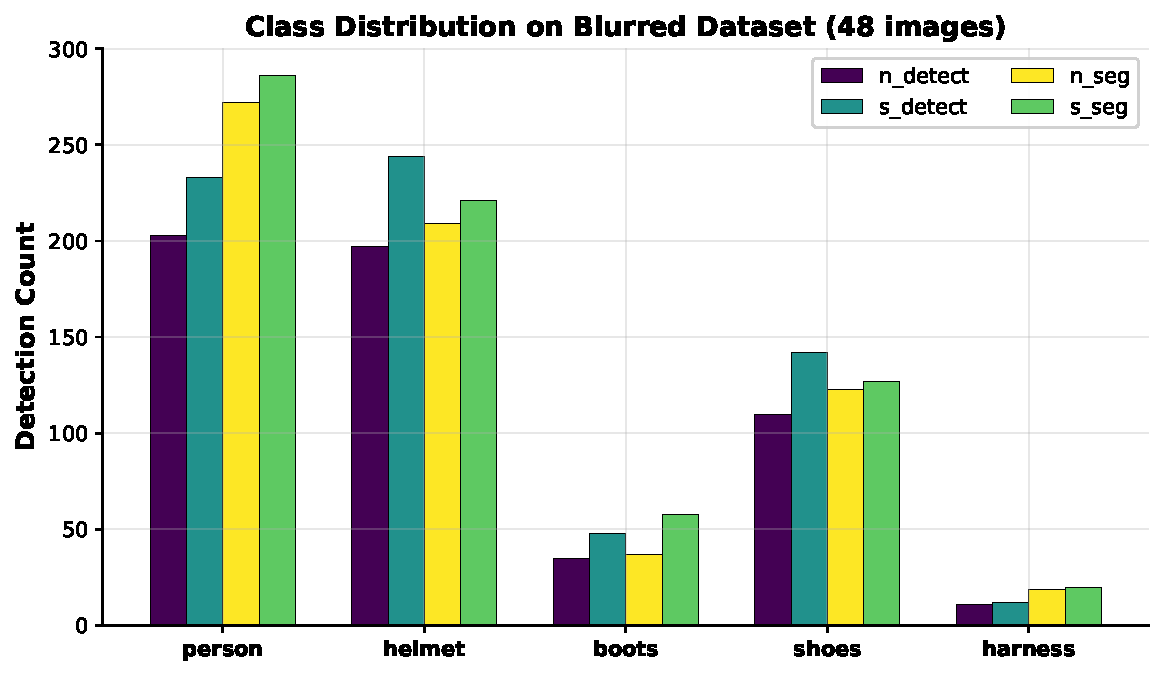
\includegraphics[width=\linewidth]{blurred_class_dist.pdf}
  \caption{Class distribution ของ detection บน blurred dataset}
  \label{fig:blurred_cls_dist}
\end{subfigure}\hfill
\begin{subfigure}{0.48\textwidth}
  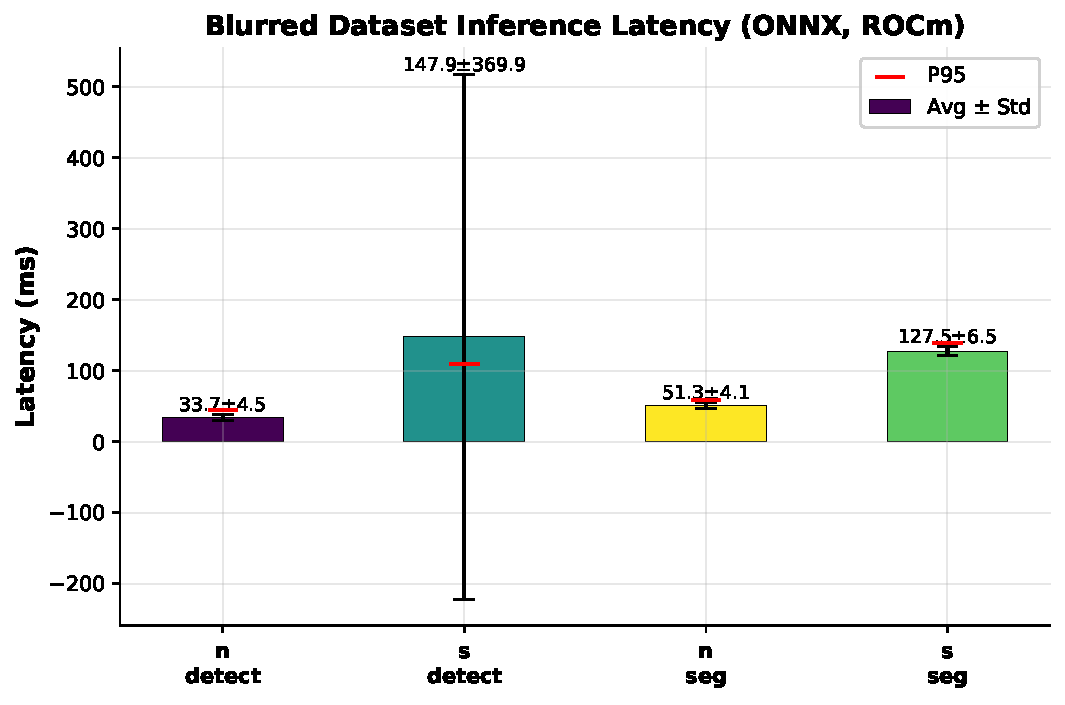
\includegraphics[width=\linewidth]{blurred_latency.pdf}
  \caption{Latency พร้อม std error bar และ P95 marker}
  \label{fig:blurred_lat}
\end{subfigure}
\caption{สถิติการ inference บน blurred dataset (48 ภาพ) ด้วย ONNX: (a) class distribution แสดงว่า person และ helmet ถูกตรวจจับได้มากสุด ส่วน harness น้อยสุด (b) latency แสดงว่า n\_detect เร็วสุดและ stable ส่วน s\_detect มี variance สูง}
\label{fig:blurred_stats}
\end{figure}

\section{Good Cases (หลาย class, หลาย detection)}

\begin{figure}[H]
\centering
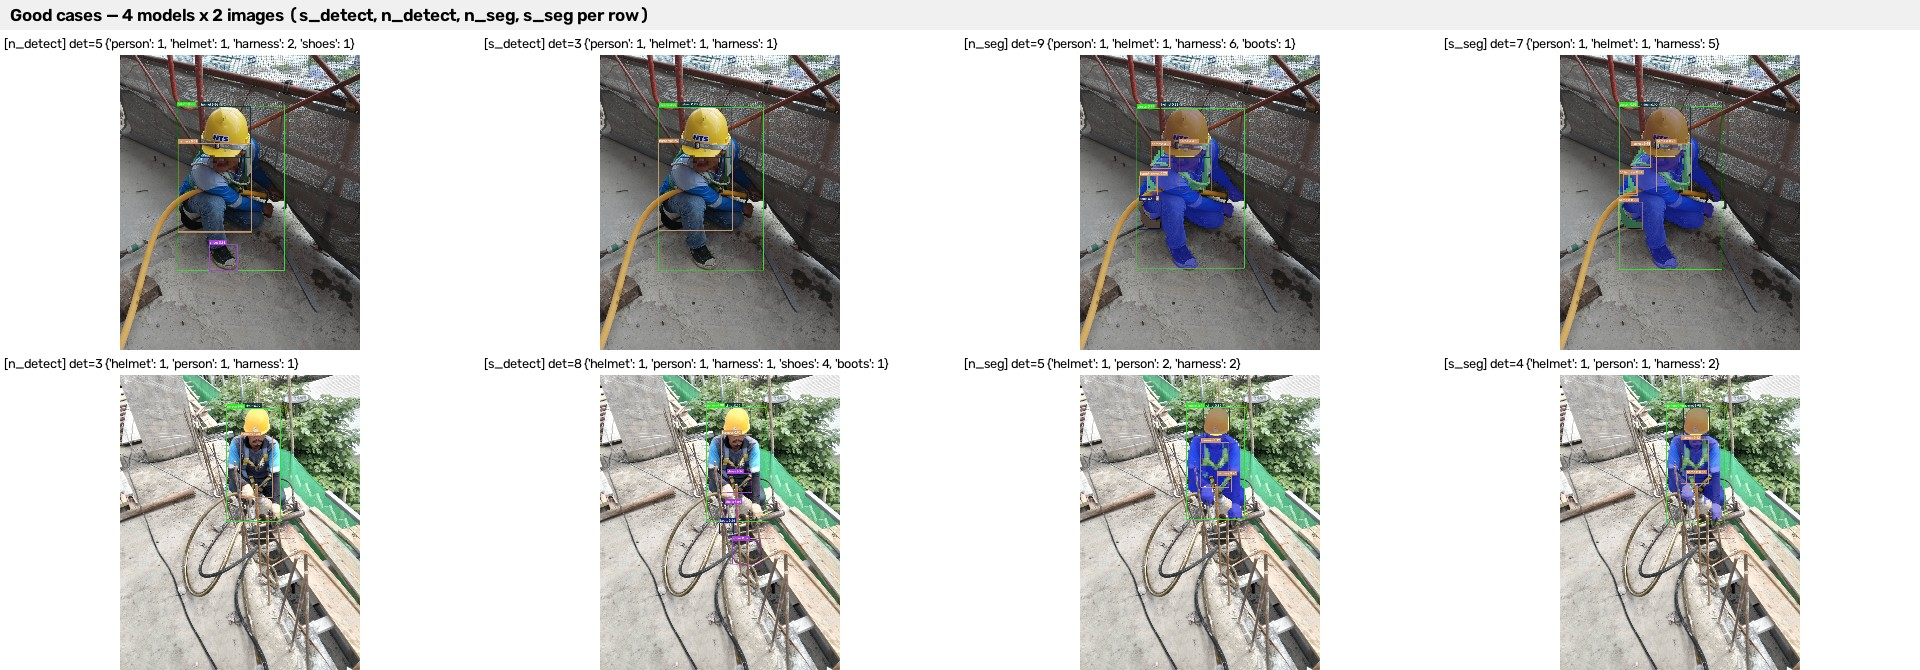
\includegraphics[width=\textwidth]{figures/blurred/blurred_good_montage.jpg}
\caption{Good cases บน blurred dataset — 2 ภาพที่ตรวจจับได้ครบทุก class (5 classes) แสดงผล 4 โมเดล side-by-side — กรอบสี = bbox, พื้นหลังสีโปร่ง = mask (seg models) — สีตาม SAM perceptual colormap (LAB kmeans, seed=42) — แถวบน: n\_detect, s\_detect, n\_seg, s\_seg สำหรับภาพที่ 1 แถวล่าง: สำหรับภาพที่ 2}
\label{fig:blurred_good}
\end{figure}

\section{Bad Cases (น้อย class, น้อย detection)}

\begin{figure}[H]
\centering
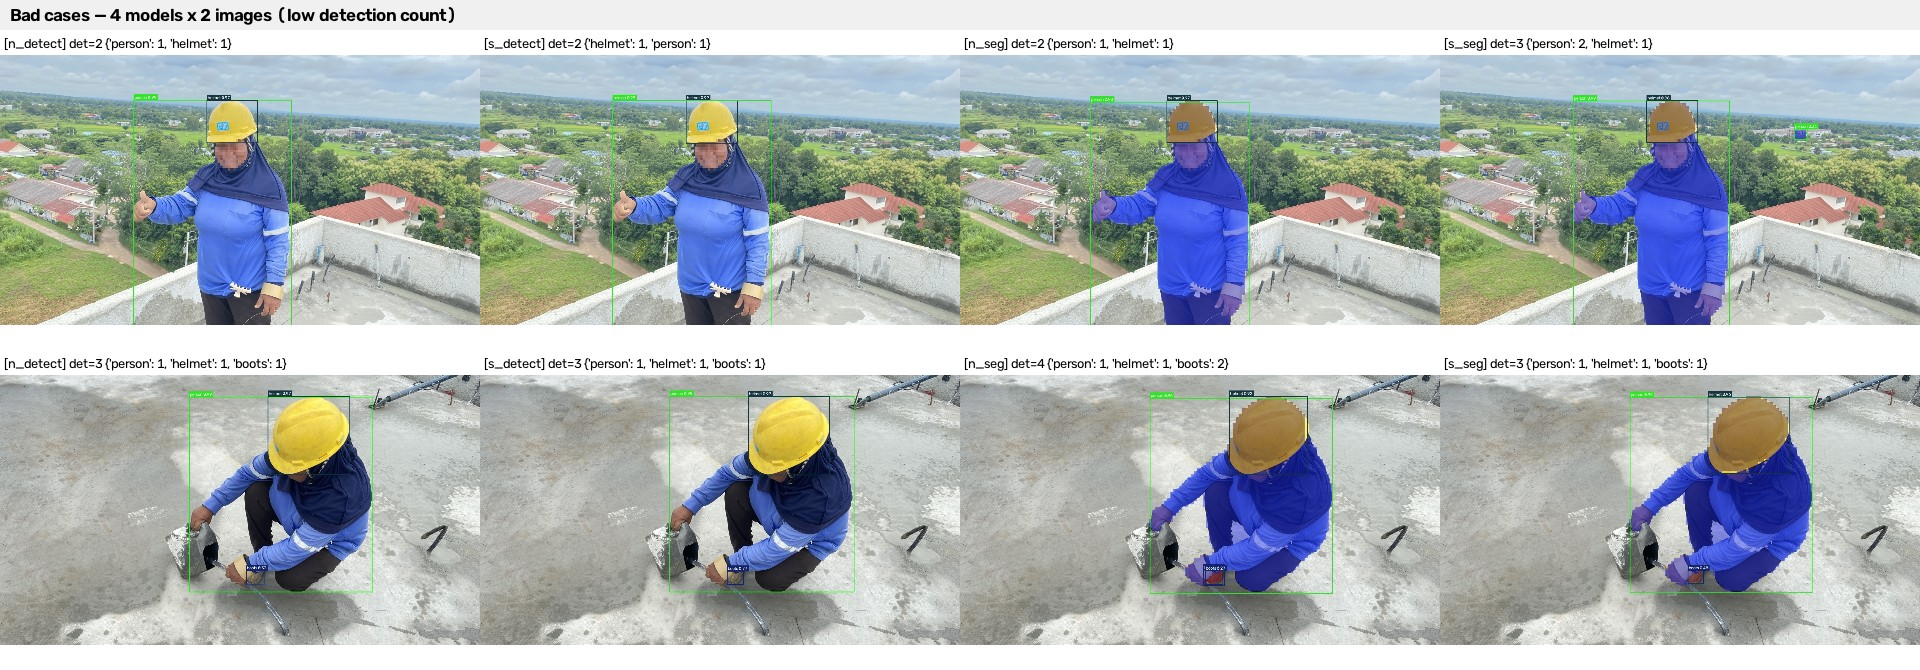
\includegraphics[width=\textwidth]{figures/blurred/blurred_bad_montage.jpg}
\caption{Bad cases บน blurred dataset — 2 ภาพที่ตรวจจับได้น้อยที่สุด (9--13 รายการ, 2--3 classes) แสดงผล 4 โมเดล side-by-side — สังเกตว่าโมเดลยังตรวจจับ person และ helmet ได้ แต่พลาด boots, shoes, harness ในภาพ blur จัด — แสดงว่าโมเดลยังขาด robustness ต่อ blur สำหรับวัตถุขนาดเล็ก}
\label{fig:blurred_bad}
\end{figure}

\section{Per-Model Top Detections}

\begin{figure}[H]
\centering
\begin{subfigure}{0.48\textwidth}
  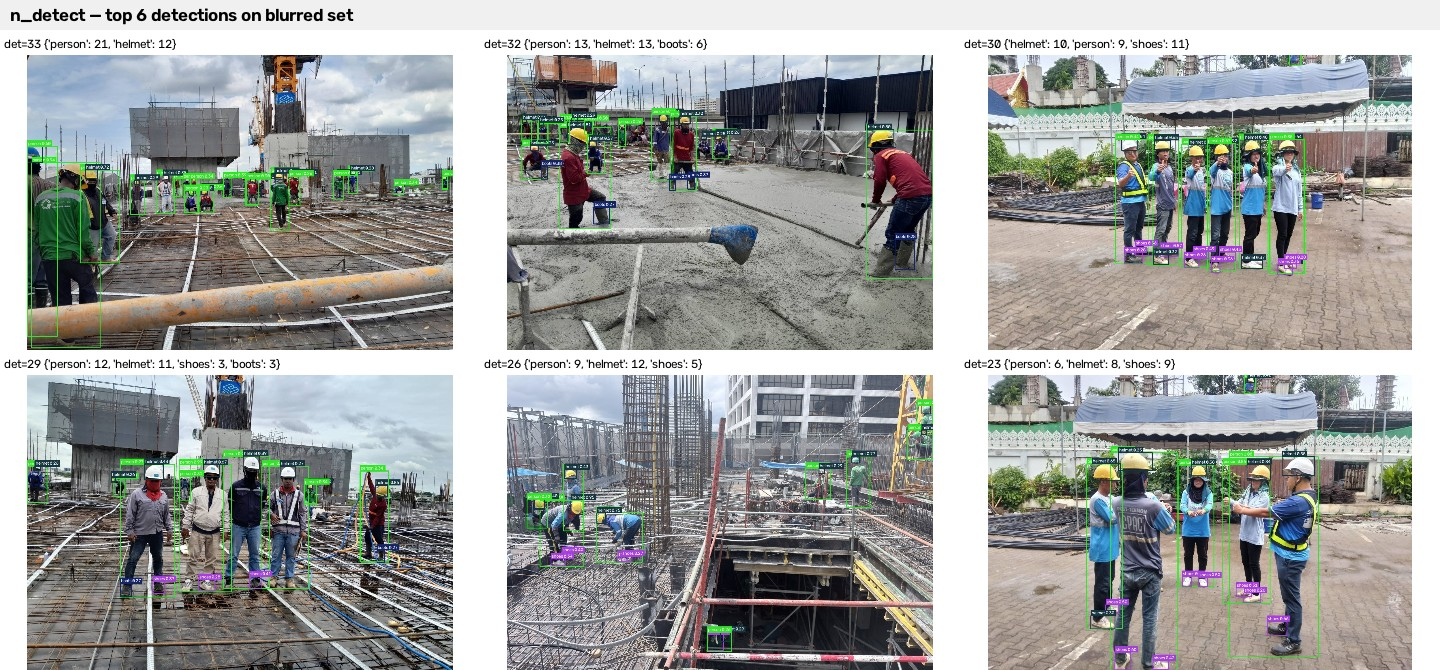
\includegraphics[width=\linewidth]{figures/blurred/blurred_n_detect_top6.jpg}
  \caption{n\_detect (bbox only)}
  \label{fig:blurred_n_det}
\end{subfigure}\hfill
\begin{subfigure}{0.48\textwidth}
  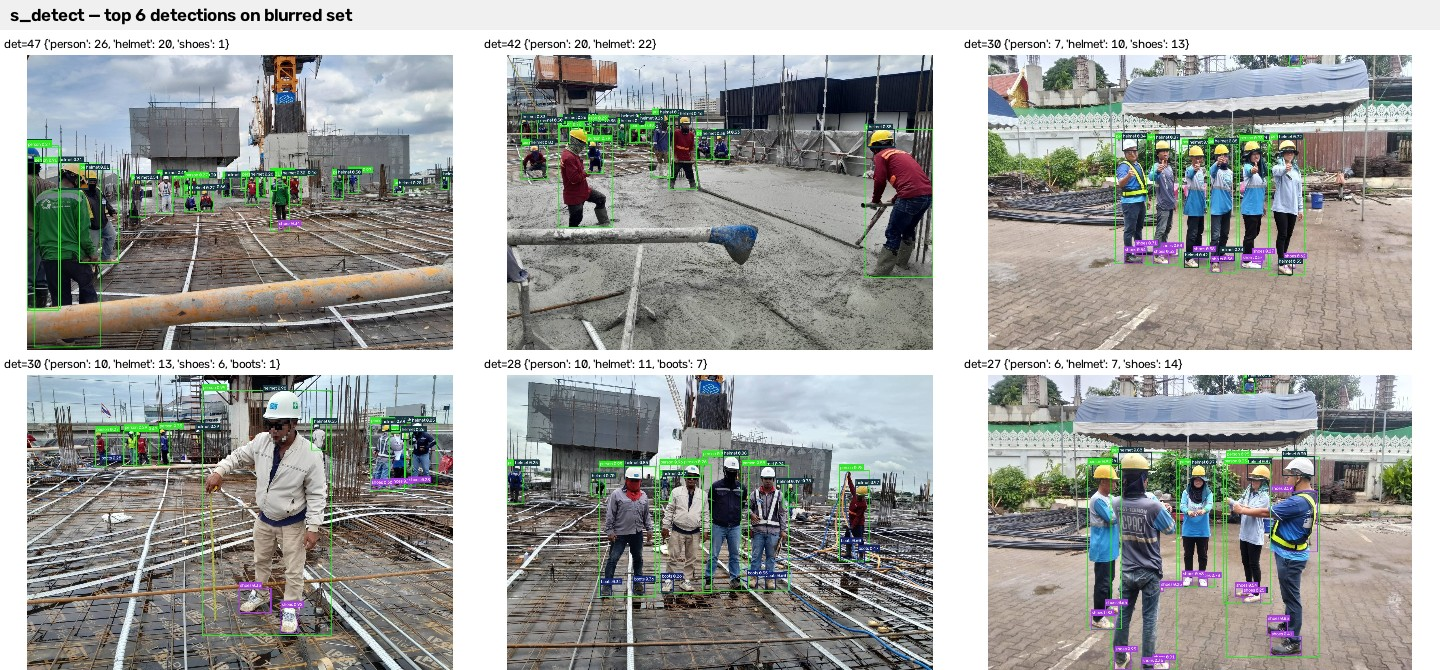
\includegraphics[width=\linewidth]{figures/blurred/blurred_s_detect_top6.jpg}
  \caption{s\_detect (bbox only)}
  \label{fig:blurred_s_det}
\end{subfigure}

\begin{subfigure}{0.48\textwidth}
  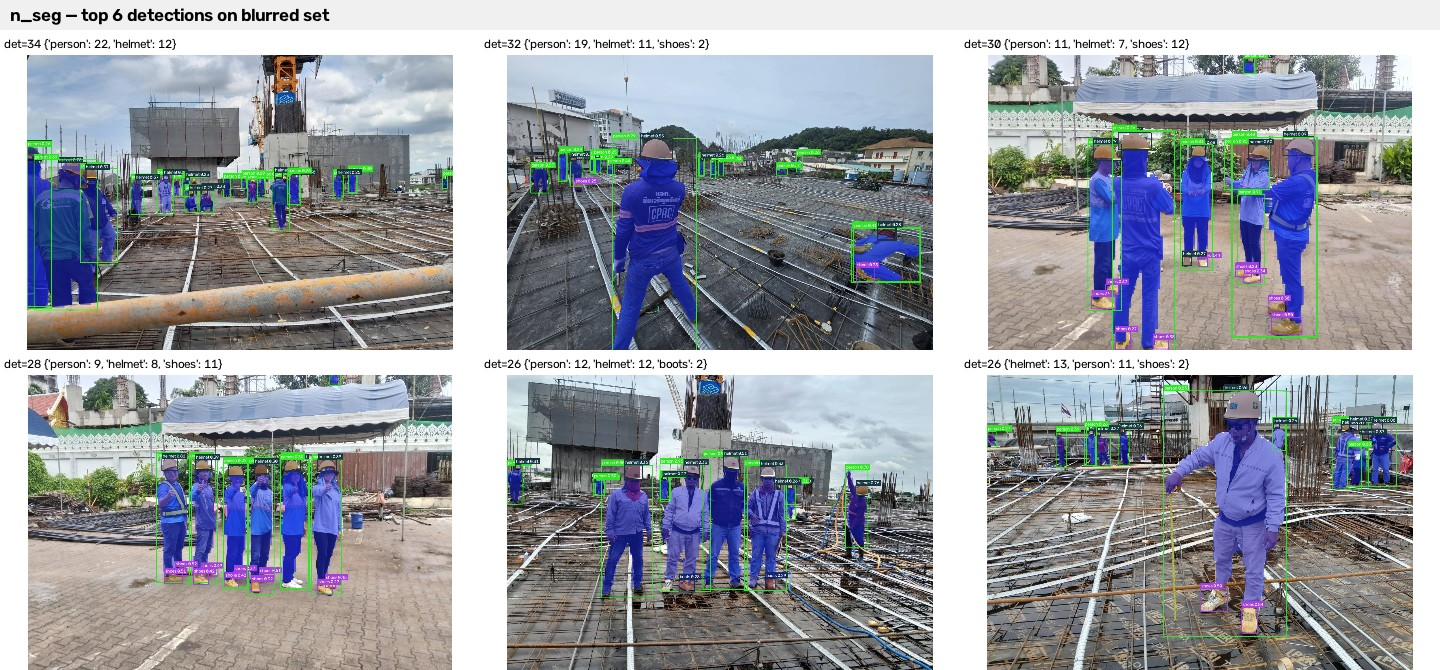
\includegraphics[width=\linewidth]{figures/blurred/blurred_n_seg_top6.jpg}
  \caption{n\_seg (mask + bbox)}
  \label{fig:blurred_n_seg}
\end{subfigure}\hfill
\begin{subfigure}{0.48\textwidth}
  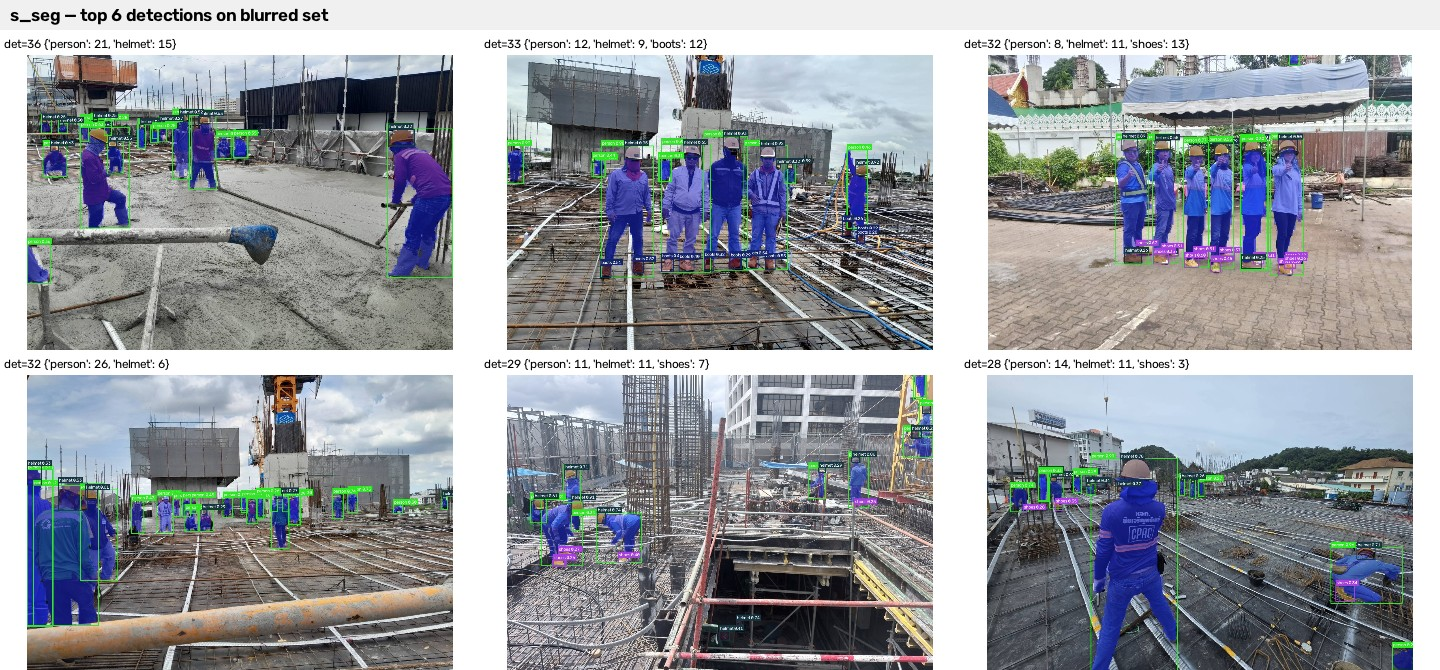
\includegraphics[width=\linewidth]{figures/blurred/blurred_s_seg_top6.jpg}
  \caption{s\_seg (mask + bbox)}
  \label{fig:blurred_s_seg}
\end{subfigure}
\caption{6 ภาพที่ตรวจจับได้มากที่สุดบน blurred dataset สำหรับแต่ละโมเดล: (a) n\_detect (b) s\_detect (c) n\_seg (d) s\_seg — detect models แสดง bbox เท่านั้น ส่วน seg models แสดง mask overlay (สีโปร่ง) พร้อม bbox — สีตาม class: person, helmet, boots, shoes, harness}
\label{fig:blurred_per_model}
\end{figure}

\section{สรุป Blurred Dataset}

\begin{itemize}[leftmargin=1.5cm, itemsep=4pt]
  \item โมเดลทั้ง 4 ตัวยังทำงานได้บนภาพ blurred (0 zero-detection จาก 48 ภาพ)
  \item s\_seg ตรวจจับได้มากที่สุด (712 รายการ) แต่ช้าที่สุด (127.5 ms)
  \item n\_detect เร็วที่สุด (33.7 ms) เหมาะกับ real-time แต่ตรวจจับน้อยสุด (556 รายการ)
  \item harness ยังเป็น class ที่ยากที่สุด (11–20 รายการจาก 556–712 รายการทั้งหมด)
  \item ในภาพ blur จัด โมเดลพลาด boots, shoes, harness แต่ยังจับ person, helmet ได้
  \item ข้อแนะนำ: ถ้าต้องการ robustness ต่อ blur ควรเพิ่ม augmentation แบบ motion blur + gaussian noise ใน training set
\end{itemize}

\end{document}